\documentclass[11pt,twocolumn]{article}
\usepackage{fontspec}
\usepackage[margin=0.85in]{geometry}
\usepackage{amsmath,amsthm,amssymb}
\usepackage{graphicx}
\usepackage{booktabs}
\usepackage[authoryear,round]{natbib}
\usepackage[font=small,labelfont=bf]{caption}
\usepackage{microtype}
\usepackage[hidelinks,breaklinks=true]{hyperref}

\title{FreshCredit: Credit as Trust Quantified\\[4pt]
  \large\itshape A whitepaper on the financial application of a companion measurement protocol}
\author{Devon Shigaki~(ORCID: 0009-0003-8977-8010)\\
\small The FreshCredit Lab --- Independent Research\\
\small Correspondence: freshcredit.xyz}
\date{}

% --- Float-page layout tuning: reduce white bands on float-dense pages ---
\renewcommand{\topfraction}{0.85}
\renewcommand{\bottomfraction}{0.70}
\renewcommand{\textfraction}{0.10}
\renewcommand{\floatpagefraction}{0.60}
\renewcommand{\dbltopfraction}{0.80}
\renewcommand{\dblfloatpagefraction}{0.55}
\setcounter{topnumber}{3}
\setcounter{bottomnumber}{2}
\setcounter{totalnumber}{5}
\raggedbottom


\begin{document}
\makeatletter
\twocolumn[\begin{@twocolumnfalse}
\maketitle
\begin{abstract}
Credit is the largest-scale compliance measurement in the economy --- and, on the stack's {[HYPOTHESIS]}-labeled bridge (\S~2.2: the score's contract-enforced inputs are assurance-channel validations whose correlation with trustworthiness is hypothesized, not identical to it), its trust-quantified projection. It is performed by a centralized architecture that mismeasures in every documented direction: it excludes tens of millions of creditworthy people, tolerates error rates that regulators sanction, loses the data of hundreds of millions, and charges the measured for the privilege. FreshCredit is the financial application of a companion measurement protocol: it points the protocol's domain-agnostic trust-measurement stack at financial validation streams and rebuilds the credit pipeline --- Report $\rightarrow$ Score $\rightarrow$ Offer --- as the externalization of the biological expectation--validation loop. The design commitments are three: (i) dual measurement layers --- a financial stream (consumer-permissioned cash-flow, binary validations on a shared monetary baseline) and a physiological stream (HRV, sleep, activity) that is scored against the biological theory for theory validation and is structurally excluded from credit decisions; (ii) user-owned records --- database-per-tenant storage with selective-disclosure credentials, so the measurement no longer requires surveillance; and (iii) verified feedback --- every validation settles on-chain and is light-client verifiable by the user. All financial statistics cited here are regulator- or primary-source verified where cited as fact; vendor-reported figures are labeled as such. The complaint-database statistics are stated against their exact counting base; benchmark figures cited in print are frozen, dated snapshots, and the live calculator at freshcredit.xyz/cost is a supplementary tool, not a reference; all modeled projections are labeled as projections. This document contains all of the stack's financial content; the companion protocol preprint contains none.
\end{abstract}
\smallskip\noindent \textbf{Keywords:} credit; trust quantified; cash-flow underwriting; user-owned records; selective-disclosure credentials; on-chain settlement; measurement without surveillance
\vspace{1.2em}
\end{@twocolumnfalse}]
\makeatother

\textbf{Epistemic labels used in this document:} [DERIVED], [STANDARD] (textbook results derived for self-containment), [ANALOGY], [HOMOLOGY], [EMPIRICAL], [HYPOTHESIS], [SIMULATION]. Simulation identifiers follow the stack-wide registry: this paper's own simulations are "Sim W\ldots{}"; companion preprints' simulations are cited as "Sim P1\ldots{}P8", "Sim G\ldots{}", and "Sim D\ldots{}" per the stack-wide registry. The symbol convention is fixed stack-wide: \textbf{$\varepsilon_t := V_t - E_t$} (validation minus expectation; positive $\varepsilon$ is a confirmation), and the normalized mismatch $\tilde{\varepsilon} = (V - E)/s_d$ (per-domain scale $s_d$ = RMSE of the expectation distribution) is the dimensionless quantity entering all dynamics.

\medskip
\noindent\textbf{Contents}\\[3pt]
{\small\noindent
0. Hypotheses\\
1. The Problem: A Failing Measurement\\
2. Why Financial Data Is the Cleanest Validation Stream\\
3. The Architecture: The Companion Measurement Protocol Configured for Financial Validation Streams\\
4. Benchmarks and Projections (Discipline)\\
5. Regulatory Posture (as of September 2026)\\
6. Alignment: The Stack in One Line\\
}
\medskip

\begin{equation}
\varepsilon_t := V_t - E_t, \qquad \tilde{\varepsilon} = \frac{V - E}{s_d}
\label{eq:epsilon}
\end{equation}

\section*{0. Hypotheses}

\textbf{Null hypothesis ($\mathrm{H}_0$).} Isolated, user-owned databases do not reduce attack surface or friction in credit access, and edge architecture does not unlock inclusion for thin-file populations.

\textbf{Alternative hypothesis ($\mathrm{H}_1$).} Isolated per-user databases reduce breach blast radius (variance reduction, not elimination --- win region $p_{\mathrm{device}} + p_{\mathrm{commonmode}} < p_{\mathrm{org}}$) and reduce observation salience (the surveillance-bias leg stands on the Penney-class evidence; demand-characteristics evidence is heterogeneous with frequent nulls); edge architecture enables participation for credit-invisible and thin-file populations; and financial data synchronization produces higher-fidelity trust measurement than centralized alternatives [HYPOTHESIS --- the concordance pilot of \S~3.4 is the registered test; in-silico pipeline validation only].

\textbf{Proof obligations:} (1) attack-surface reduction --- per-tenant isolation caps breach blast radius structurally (Section 1.3 documents the centralized failure record; \S~4.3 states the expected-loss model in full, including the endpoint-multiplication and key-loss counter-terms); (2) friction reduction --- on-device verification against bureau-mediated delay; (3) inclusion --- thin-file borrowers become measurable through permissioned cash-flow (Sections 1.1, 2), benchmarked against the incumbent alternative-data products that have already moved part of this population (\S~2.3); (4) cost --- the cost-of-engagement reduction targeted by the companion protocol preprint's $\mathrm{H}_1$, with like-for-like marginal-cost accounting in print and the live calculator maintained as a supplementary tool (Section 4); (5) signal fidelity --- dual financial + physiological measurement validates the biological stage structure without physiology entering decisions, including an explicit analysis of the fused-estimator leakage channel (Section 3.2).

\section*{1. The Problem: A Failing Measurement}

\subsection*{1.1 Exclusion --- the measured population is a subset of the trustworthy population}

A measurement product cannot afford stale measurement, so this paper works on the CFPB's corrected frame throughout. The Bureau's 2015 estimate (26 million U.S. consumers credit invisible; 19 million unscorable) was revised by its own June 2025 technical correction after one bureau's submissions were found to have excluded whole record categories (files containing only deferred student loans, collections, or closed accounts): the corrected 2010 estimate is 13.5 million invisible (5.8\% of adults) alongside 29.7 million unscored (12.7\%), and the corrected 2020 benchmark is \textbf{7.0 million invisible (2.7\%) plus $\sim$25.3 million whose files are too thin or stale to score (9.8\%)} --- roughly 32 million adults outside scorable credit, even as the scored share rose from 81.6\% (191.3M) to 87.5\% (225.3M) over the decade (CFPB, 2025 technical correction). The net effect of the correction is compositional, not redemptive: the total limited-credit-history population barely moved; the invisible/unscored boundary moved. Nobody became visible.

The problem's composition, not just its size, is diagnostic: the frontier failure is no longer file creation but file \emph{sufficiency} --- records exist; reportable activity doesn't. An industry re-estimation on the pre-correction frame placed the figures higher (28 million invisible, 21 million unscorable --- 49 million; Oliver Wyman/Experian, 2022); that frame is superseded by the CFPB correction and is cited here only as the pre-correction estimate, with its demographic detail retained because the correction does not speak to it: invisibility concentrated among Black (28\%) and Hispanic (26\%) consumers versus 16\% of White and Asian consumers, and 40\% of invisibles under 25. Where the two frames disagree on market size, this document uses the corrected CFPB figures everywhere (see \S~3.3). The persistent disagreement about how many people the system fails to see is itself evidence about the measurement.

The exclusion is not a U.S. anomaly; it has a global precursor. 85\% of the world's population --- 6.7 billion people --- lives on less than \$30 per day (Our World in Data, 2023), and economies at that income level run predominantly on cash. Cash settles obligations but generates no bureau-visible history: every repaid informal loan, every settled supplier debt, every honored commitment in a cash economy evaporates at the point of settlement. Global account ownership has reached 78.7\% (World Bank Findex, 2025), but holding an account is not holding a tradable credit history --- the account is a rail, not a record of trustworthiness. The causal chain --- poverty $\rightarrow$ cash-dominant economic life $\rightarrow$ measurement invisibility $\rightarrow$ exclusion from formal credit --- means the unmeasured population is not a residual category but the global majority [EMPIRICAL for the income and account figures; the chain itself is a stated inference]. Public credit-registry coverage of adults ranges from 64\% across OECD countries to 7\% in Sub-Saharan Africa (World Bank, 2019), and scoring presupposes reporting --- there is no score without a record --- so populations outside the reporting perimeter are not poorly measured; they are unmeasured.

\subsection*{1.2 Error --- the measurement is often wrong, and correction is adversarial}

The FTC's congressionally mandated accuracy study found 26\% of consumers identified at least one potentially material error on a credit report, 21\% had an error corrected after dispute, 13\% experienced a credit-score change from corrections, and 5\% had errors serious enough that the uncorrected file placed them in a worse credit-risk tier than the corrected one (equivalently, 5.2\% moved to a better --- lower-risk --- tier post-correction) (FTC, 2013); the 2015 follow-up found that while 80\% of disputing consumers received some modification, only 37\% received all requested modifications, and of consumers with unresolved disputes $\sim$70\% still believed the disputed information was inaccurate (FTC, 2015).

Consumers register the failure at scale. In 2024 the CFPB received approximately 3.19 million complaints, of which about 2.70 million (85\%) concerned credit or consumer reporting, and more than 2.51 million ($\sim$93\% of those) named Equifax, Experian, or TransUnion (CFPB Consumer Response Annual Report, May 2025). What the complaints are \emph{about} is answered on a different, explicitly stated base --- the CFPB's public Consumer Complaint Database, which publishes fewer complaints than it receives: of the 2,365,586 published credit-reporting complaints received in 2024, \textbf{"incorrect information on your report" accounts for 1,175,009 (49.7\%) and "problem with a company's investigation into an existing problem" for 455,637 (19.3\%) --- together 69.0\% of published credit-reporting complaints in the database (sum of the rounded shares; exact 68.93\%)} (CFPB Consumer Complaint Database, queried 2026; database counts differ from total receipts because not all complaints are published, and the shares do not transfer to the 2,703,400 received base, on which they are 60.3\%). That is, on the database base, roughly 69\% of credit-reporting complaints concern report errors and the failure to correct them. The trend figures are stated as raw intake-volume facts, with the composition confound named: the 2024 volume of the incorrect-information issue ran \textbf{+247\% above the prior two years' monthly average} (CFPB, 2025); in 2025 credit/consumer-reporting complaints reached 5,806,800 --- 88\% of a near-doubled 6,635,400 total, with 5,102,800 naming the three nationwide bureaus (CFPB Consumer Response Annual Report, March 2026); and the FCRA \S~611(e) report records complaints against the three NCRAs running roughly \textbf{+3,000\% above January 2020 levels} over January 2024--June 2025 (CFPB, December 2025). Two confounds bound the interpretation: (i) the issue labels are self-classified by complainants, not adjudicated; (ii) intake volume is not verified-harm volume --- the Bureau's $\sim$3\% figure for potentially unauthorized third-party submissions bounds only \emph{unauthorized} third parties, and authorized dispute-mill volume is unbounded by it. Consumers had already attempted to resolve the issue directly with the company in 86\% of closed complaints --- the complaint data captures the failed correction loop, not first contact. In January 2025 the CFPB ordered Equifax to pay \$15 million for improper dispute investigation; in 2023 it ordered TransUnion to pay \$23 million for illegal practices. The failure is institutional, not incidental: in 2017 Moody's --- one of the three dominant credit rating agencies --- formally acknowledged deviating from its own published rating methodologies under issuer-pay conflicts of interest in the run-up to the financial crisis, and settled with the U.S. Department of Justice, 21 states, and the District of Columbia for nearly \$864 million (U.S. DOJ, 2017). Centralized scoring institutions have a documented record of compromising the measurement itself when the measurement is their product.

The error prevalence is corroborated by a second, independent instrument: the 2024 Consumer Reports/WorkMoney Credit Checkup (4,300+ volunteer participants) found 44\% of consumers who successfully checked their reports discovered at least one error, 27\% found debt-related errors serious enough to damage creditworthiness, and 25\% of would-be participants could not access their own reports at all (Consumer Reports, 2024 --- volunteer sample, not nationally representative; cited alongside the FTC's representative 2013 estimate of 26\%, which it corroborates at double the rate a decade later). The share of applicants plausibly losing approvals or pricing to measurement error can be bounded [DERIVED]: the lower bound is the FTC's representative 5\% (errors serious enough to worsen loan terms); the upper bound is the Credit Checkup's 27\% (volunteer sample, debt errors affecting creditworthiness); a midpoint derivation --- roughly one-third of the 44\% who find errors facing decision-relevant issues --- yields $\sim$13--15\% of applicants. This is a derived estimate from two instruments with different sampling frames, not a measured rate, and is presented as such.

The market itself renders the same verdict, and here the evidence is regulatory rather than rhetorical. The U.S. credit-repair industry --- whose product is navigating the incumbent's error-correction process on consumers' behalf --- is a $\sim$\$6.8 billion sector with $\sim$25,000 businesses (IBISWorld, 2026 estimate). Its largest brands were the subject of the CFPB's largest-ever victims'-relief distribution: in \emph{CFPB v. PGX Holdings/Progrexion} (Lexington Law and CreditRepair.com), a March 2023 district-court ruling found illegal advance fees under the Telemarketing Sales Rule and deceptive marketing under the CFPA, producing a $\sim$\$2.7 billion judgment and a 10-year telemarketing ban; the companies entered Chapter 11 and shut $\sim$80\% of operations, and in December 2024 the CFPB distributed \textbf{\$1.8 billion to $\sim$4.3 million harmed consumers} (CFPB, 2024). A sector of that size and that enforcement record would have no demand if the measurement were accurate and correction workable. The CFPB notes that credit-repair organizations now submit complaints at scale --- though the Bureau itself flagged only $\sim$3\% of 2024 credit-reporting complaints as potentially submitted by unauthorized third parties (per NCLC, 2026), and 86\% of complainants had already attempted resolution directly with the company; the industry's existence is the signal, its submission volume the same signal amplified, and its standardized dispute spam is itself documented to degrade bureau response quality --- a downstream symptom of the failure, not an artifact that explains the complaint data away.

The measurement is also expensive to rent: lender-paid tri-merge report bundles have risen from $\sim$\$15/\$30 (single/joint) to \textbf{\$50--\$110+ per pull} in two years (CFPB, 2024 RFI on mortgage closing costs; CHLA, 2024), and amortized across applications that never close, total credit costs per closed loan reached \textbf{\$510--\$725} (CHLA, 2024) --- a direct, rising tax on every originator, passed to borrowers. (The same per-pull and per-closed-loan figures are used in \S~4.1; this document does not mix the two bases.)

\subsection*{1.3 Breach and fraud --- the custodial model concentrates risk}

The 2017 Equifax breach exposed $\sim$147 million people and settled for at least \$575--700 million. In 2021, 23.9 million U.S. residents ($\sim$9\% of the population 16+) experienced identity theft (BJS, 2023); U.S. compromises hit a record 3,322 in 2025, and while victim notices fell to 278.8 million (-79\% YoY) that was only because 2024's six "mega-breaches" --- four of them preventable with MFA/passkeys, $\sim$85\% of that year's 1.367 billion notices --- were not repeated (ITRC, 2026; the 2024 figure is ITRC's restated value, which this document uses consistently). U.S. financial institutions spend \$5.75 per \$1 of fraud losses (LexisNexis, 2025; industry vendor study). Synthetic identity fraud --- identities "seasoned" with manufactured payment history for months to years before bust-out --- is described by the Federal Reserve's three-part white-paper series (2019--2020) and mitigation toolkit (2022) as among the fastest-growing financial crimes in the U.S., with industry estimates cited by the Fed putting unsecured-credit losses in the billions (Federal Reserve FedPayments Improvement, 2019--2022). (A widely circulated claim that "95\% of synthetic identities pass onboarding undetected," attributed to Thomson Reuters across vendor blogs, could not be traced to any primary source or methodology and is treated here as an unverifiable industry claim --- it is not used.) FBI IC3-reported losses reached \$20.9 billion in 2025 (+26\% YoY, the first year above \$20B; IC3, 2026). The attack surface is human, not infrastructural: $\sim$60\% of breaches involve the human element, with stolen credentials ($\sim$22\%), vulnerability exploitation ($\sim$20\%), and phishing ($\sim$16\%) the leading initial vectors, and third-party involvement doubling to 30\% of breaches in a single year (Verizon DBIR, 2025) --- a structural argument for verification that does not depend on custodial secrecy. The risk arithmetic --- distribution multiplies the number of attackable endpoints while dividing the blast radius of each --- is stated with base rates and a break-even condition in \S~4.3, not deferred.

\subsection*{1.4 Distortion --- surveillance changes the measured behavior}

Credit files are built from involuntary surveillance, and observed behavior is distorted behavior: population-scale chilling effects are measurable and statistically significant (Penney, 2016), and demand characteristics show heterogeneous, bidirectional participation effects with frequent nulls (McCambridge, 2014: 12 of 19 studies positive, 5 clear nulls; the review concludes little is securely known about conditions, mechanisms, or magnitudes --- the design precaution stands on the stronger Penney leg and on the generic risk; the strong empirical claim does not). The deeper structural point is the direction of the gaming incentive. Campbell's law --- the more a quantitative indicator is used for decision-making, the more it is subject to corruption pressures (Campbell, 1979) --- predicts score-targeting, and the incumbent industry demonstrates it at both ends: issuer-pay ratings agencies deviated from their own published methodologies when the indicator became the product (Moody's DOJ settlement, \S~1.2), and consumers rationally optimize the score rather than the underlying financial health. But the manipulation is asymmetric: no consumer games the system to make their measured value worse. A correction regime that penalizes positive-but-optimized behavior therefore cannot distinguish manipulation from genuine improvement and is incoherent as a remedy; the only coherent fix is to change what is measured --- from a surveilled snapshot that can be performed, to an owned, accumulating history.

That fix has a price tag, and this document states it instead of asserting it. The protocol's cost figures make manufactured history cheap in \emph{money}: at the stack's own per-event settlement cost ($\sim$\$0.001/event, x402-class) and its simulated $\sim$100.5 events per unit of standing, a synthetic history of 10 units of standing costs \textbf{\$1.01 without provider attestation} (Technical Appendix, Sim-Battery A, Study 3) --- so the claim "costly to fake" is \textbf{false in dollar terms}, and this paper does not make it. (The companion protocol preprint's Sim P8 battery prices the break/build update asymmetry that makes manufactured standing expensive to \emph{sustain} under immediate feedback; Technical Appendix, Sim-Battery A, Study 3, prices its manufacture. The Technical Appendix --- the stack's simulation batteries and mathematical development --- is bundled with the Supporting Document (deposit pending); it is cited throughout as "Technical Appendix, Sim-Battery A/B, Study N" and "Technical Appendix, \S~M".) The defense is attestation plus time, three-layered [SIMULATION]:

\begin{enumerate}
\item \textbf{Provider attestation.} Every validation event is co-signed by the counterparty/provider, multiplying per-event manufacture cost by the attestation multiplier m (m = 10/100/1000 $\rightarrow$ \$10.05/\$100.50/\$1,005 per 10 units). Cost alone is a weak deterrent at m $\leq$ 10.
\item \textbf{A wall-clock time floor --- quoted per standing level and per rate.} Attested events must occur in wall-clock time and cannot be compressed except by parallel-provider collusion (the collusion caveat, companion protocol preprint, \S~3.7); the floor for manufacturing 10 units of standing (HIGH standing, 1,005 events) is quoted per rate (Technical Appendix, Sim-Battery A, Study 3): \textbf{at $\leq$2 attested events/day: 1.4 years} (at 0.5/day: 5.5 years); \textbf{at the model's own high-standing rates (2.5--3.76 events/day, 5/day max grid): $\sim$0.55--1.1 years (0.73 yr at 3.76/day; 0.55 yr at 5/day)}; and \textbf{at the decisionable threshold ($\sim$60--70 events): $\sim$72 days with one cooperative provider}. The stack's own rate model (rate = $r_{\mathrm{floor}} + 5S$) is what generates those high-standing rates at decision-relevant standings, so the 1.4-year figure is the $\leq$2/day value, not the minimum. Security therefore rests on the attestation requirement plus provider collusion cost, with time as a secondary defense. Faking the history requires \emph{living} it --- the cost is time under observation, not dollars.
\item \textbf{Rollups decouple the honest user's cost.} Block rollups (K events per anchor at \$0.001/anchor) drop the honest user's lifetime $\sim$1,005-event anchoring cost from \$1.005 to \textbf{\$0.0001 --- a $10^{4}\times$ discount that does not touch the Sybil time floor} (Technical Appendix, Sim-Battery A, Study 3). Honest cost and attack cost are thereby decoupled by construction.
\end{enumerate}

The caveat is disclosed, not buried: the time floor assumes providers refuse to backdate signatures and that one Sybil cannot contract many providers in parallel --- \textbf{parallel-provider collusion divides the time floor by the number of colluding providers}, so the floor must be paired with a provider-diversity requirement (not yet modeled). The incumbent system faces the same attack in its own currency: tradeline rental sells authorized-user slots on strangers' seasoned accounts for \textbf{\$325--\$4,000+ per slot}, with marketing claims the FTC alleged were unsubstantiated (FTC enforcement under the Credit Repair Organizations Act), and synthetic identities are seasoned for months--years before bust-out (Federal Reserve white papers, 2019--2020). The deployed countermeasure in both systems is the same --- cross-checking against an authoritative issuer (the SSA's eCBSV consent-based SSN verification service for lenders; here, provider-signed attestation): FreshCredit's design adopts the deployed countermeasure natively rather than as an aftermarket patch.

Two disclosure obligations attach to this design. First, Campbell's law applies to FreshCredit's own score: it is a decision-relevant indicator and will attract optimization pressure --- the priced asymmetry above is the answer, and \S~4.3 carries the residual harm accounting. Second, per the stack's own measurement theory (companion theory preprint, \S~3.3), user-owned measurement drives observation salience toward its floor but not to zero --- the salience floor is nonzero, so $\psi \rightarrow \psi_{\min} < 0$ (reduced in magnitude, not eliminated; in the stack's convention $\psi$ $<$ 0 is the chilling regime), and FreshCredit's measurement still distorts, illustratively inflating mismatch variance by $\sim$5\% at residual salience $\psi = -0.05\mu$ (Technical Appendix, Sim-Battery B, Study 3). The architecture minimizes observation-driven distortion; it does not eliminate it, and no claim of $\psi$ = 0 is made.

\subsection*{1.5 The behavioral-economics diagnosis}

Centralized scoring fails human trust dynamics because humans are not the rational agents the models assume: prospect theory documents systematic loss aversion and framing effects (Kahneman, 2011; Thaler, 2015), and the companion biology preprint explains why --- surveillance and distorted framing corrupt the recognition stage of the expectation--validation loop, so people behave against the model's expectations precisely because the model's measurement conditions are adversarial. At the macro scale, economies are adaptive systems that evolve by differentiation, selection, and amplification (Beinhocker, 2006): a credit architecture that cannot adapt its measurement to new populations selects against them arbitrarily.

The stakes extend beyond loan books, and the evidence is stated here with its causal strength graded rather than inflated. Household financial behavior is associated with well-being (Bia\l{}owolski, W\k{e}ziak-Bia\l{}owolska, \& McNeely, 2021 --- longitudinal outcome-wide analysis: financial fragility and low financial control predict subsequent worse well-being). The exclusion pathway is plausibly linked to a documented clinical endpoint --- shame, withdrawal, and social isolation --- and social isolation and loneliness are \emph{associated} with elevated all-cause mortality in prospective observational cohorts: confounder-adjusted OR = 1.29 for social isolation, 1.26 for loneliness, 1.32 for living alone (Holt-Lunstad et al., 2015, meta-analysis of 70 prospective studies, 3.4M participants) --- associations in which reverse causation is not excluded, classified by the U.S. Surgeon General as a public-health epidemic (2023). Downstream of the mechanisms this paper addresses, two stronger links are documented with their evidence classes: elder financial exploitation is associated with a \textbf{300\% elevation in mortality risk} in a prospective cohort (Burnett et al., 2016) --- the strongest single observational link from financial victimization to mortality; and among identity-crime victims seeking help, \textbf{71\% report repeat victimization and 16\% report suicidal ideation against a 2--3\% historic baseline} (ITRC, 2025 --- victim-services sample, not population-representative). The debt--health link is likewise associational at the individual level: in the nationally representative NLSY79 cohort (young adults 24--32), high debt-relative-to-assets was associated with \textbf{+11.7\% perceived stress and +13.2\% depressive symptoms} versus means, and with worse self-reported health, controlling for prior health and socioeconomic status; the diastolic blood-pressure association was weaker and less robust in adjusted models (Sweet et al., 2013). Critically, the credit--health correlation is substantially confounded: in the Dunedin cohort (N = 1,037), human-capital factors (education, cognition, self-control) explain \textbf{$\sim$45\% of the credit-score--cardiovascular-risk association} (Israel et al., 2014, PNAS) --- third factors, not credit denial, do much of the work. The nearer-causal identifications come from adjacent shocks, not from score denial itself: zip-level foreclosure spikes produce significant increases in urgent hospitalizations, including for preventable and mental-health conditions (Currie \& Tekin, 2015, quasi-causal fixed-effects design); Chapter 13 bankruptcy protection \emph{increases earnings and decreases mortality} under a judge-leniency instrument (Dobbie \& Song, 2015); and Medicaid expansion cut medical-debt flow into collections by 34 percentage points relative to non-expansion states (Kluender et al., 2021, diff-in-diff). Accordingly, this document does \textbf{not} claim the incumbent system "is a morbidity exposure." The defensible statement is narrower and still serious: credit exclusion sits upstream of documented financial shocks (foreclosure, unmanageable debt, medical collections) that carry quasi-causal morbidity and mortality signatures, and the associational links from debt to stress, depression, and isolation are measured at population scale.

The loss-of-opportunity framing is the better-evidenced channel, and it is stated as such: credit and liquidity constraints bind on human-capital investment --- \$10,000 of additional liquid housing wealth raises college enrollment by $\sim$0.7--0.9 percentage points (Lovenheim, 2011) and shifts enrollment toward flagship institutions while raising completion for low-income students (Lovenheim \& Reynolds, 2013, plausibly exogenous housing-boom variation); 17.8\% of credit-report holders carried medical debt in collections in June 2020 (Kluender et al., 2021). Exclusion from measurement is exclusion from education, housing, treatment, and food-security margins where credit access is the binding constraint --- that is the documented cost this product exists to reduce.

Two measurement-vocabulary disciplines are applied throughout this document, because the incumbent literature routinely blurs them. \textbf{Incidence vs. prevalence.} Identity theft and data breaches are incidence --- event rates per period (23.9M U.S. victims in 2021; 3,322 compromises in 2025). Poor financial education, thin files, and exclusion are prevalence --- chronic stocks carried across years. The two have different remedies, and both are biased by the same two mechanisms: stigma suppresses reporting, and record-keeping gaps suppress measurement. The stigma channel is quantified: two in three indebted consumers minimize or hide their debt (Self Financial company survey, n = 1,078, 2025 --- vendor-reported, not independently validated), 95\% of bankruptcy filers report shame and 80\% actively conceal the filing (Thorne \& Anderson, 2006), shame is not only a reporting bias but a hardship mechanism --- across a study program totaling N = 9,110, financial shame drives disengagement from one's finances, which worsens hardship and thereby deepens shame in a self-reinforcing spiral (Gladstone, Jachimowicz, Greenberg, \& Galinsky, 2021) --- and the resulting silence starves the research field itself --- financial distress is under-discussed at both ends of the wealth scale, for opposite reasons (shame below, taboo above), so the true distribution of harm is systematically under-sampled exactly where it is largest. This is a structural argument for the architecture, not a footnote: a private, user-owned record at the edge lets a person engage with their own data without disclosure, reducing stigma-driven signal bias at the source while improving record-keeping completeness. \textbf{Risk language.} Where effects are quantified we report relative risk alongside absolute risk differences, and --- following diagnostic convention --- specificity before sensitivity, with predictive values always stated against their prevalence (the base-rate dependence is computed from Bayes' rule plus Monte Carlo in Sim W1 --- not demonstrated on real credit data: the same instrument's PPV falls from 0.47 at 22\% prevalence to 0.03 at 1\% --- reproduced exactly in the re-run, Figure 9). The promised number-needed-to-harm accounting is performed in-paper in \S~4.3 (fees, key loss, consent fatigue, cold start), not deferred. No case-fatality analog exists for trust collapse; mortality and morbidity are the correct endpoints, and they are reported with their causal grades attached.

\subsection*{1.6 The Solution: The Edge Is Now Cheaper, Faster, and Safer}

Three problems that once forced centralization are now solved problems, and their solutions compose:

\begin{itemize}
\item \textbf{Orchestration.} Database-per-tenant operation at consumer scale is a solved operational pattern: embedded-replica databases (libSQL/Turso) give each user an isolated, encrypted, edge-resident store with centralized schema management --- millions of independent databases administered as one fleet (Turso's platform is explicitly designed for database-per-tenant; reads are served from the local replica with read-your-writes semantics, writes route to the primary, and cross-replica consistency is eventual --- a stated property, not a hidden one).
\item \textbf{Incentive.} Per-interaction settlement is solved by micropayment rails (x402: 100M+ payments processed in its first $\sim$6 months --- 169M+ payments in year one per Coinbase --- with sub-cent settlement on Layer-2; incubated by Coinbase, co-founded as a foundation with Cloudflare, and moved under the Linux Foundation in April 2026 with members including AWS, Anthropic, Circle, Google, Microsoft, Stripe, and Visa; early volume was inflated by memecoin-mint and retry traffic, a caveat this document carries). These rails make it economically viable to compensate validation events individually rather than monetizing aggregated surveillance.
\item \textbf{Compute.} Verification is solved at the edge: light clients (Smoldot) let any consumer device verify its own record's integrity against the audit chain without trusting a full node, and edge-compiled models evaluate trust-weighted utility locally --- no raw-data round trip to a custodian.
\item \textbf{Custody.} User-held keys no longer mean lose-your-key, lose-your-identity. Smart-account standards (ERC-4337, deployed 2023; EIP-7702, live with Ethereum's 2025 Pectra upgrade) provide guardian-quorum social recovery, scoped session keys, and key rotation, and passkey signers (WebAuthn) replace seed-phrase custody with device biometrics. Recovery and delegation are solved at the account layer without reintroducing a custodian --- removing the last structural objection to sovereign storage. The residual risks of that recovery layer --- SIM-swap of guardian contacts, guardian-service compromise, key stranding --- are priced in \S~4.3, not waved away.
\end{itemize}

The consequence inverts the incumbent economics --- conditional on attestation pricing staying well below the $m \approx 1{,}000$ break-even of \S~4.3 (mandatory attestation is the dominant fee channel there, the cost channel is net-negative at $m = 1{,}000$, and realistic attestation pricing is an open market question): centralized custody is no longer the cheap way to measure trust; it is the expensive, slow, and breach-prone way. The companion protocol preprint specifies the V1$\rightarrow$V3 architecture generations that exploit this inversion --- sovereign storage, verifiable settlement, frictionless engagement; FreshCredit consumes that protocol unchanged.

\subsection*{1.7 Credit as a hub-concentrated, heavy-tailed system}

Credit is the trust-mediated layer of the transaction economy. An economy is the sum of its transactions; every transaction is settled in money or credit; credit is created whenever a lender accepts a borrower's promise --- and, once created, immediately exists as both an asset and a liability; and because one participant's spending is another's income, credit-driven spending propagates self-reinforcingly through the network of incomes, producing the short (5--8 year) and long (75--100 year) debt cycles that dominate macroeconomic fluctuation (practitioner exposition: Dalio, \emph{How the Economic Machine Works}, 2013). The magnitudes establish the stakes: U.S. credit outstanding is on the order of tens of trillions of dollars, and most of what circulates as "money" is credit rather than physical currency (Dalio's framing); globally, fixed-income markets stood at \$160.7 trillion against \$157.8 trillion in equity market capitalization at end-2025 (SIFMA, 2026) --- the credit layer is at parity with the equity layer in size.

The network structure follows from the mechanism. Credit relationships form by preferential attachment to perceived trustworthiness [HYPOTHESIS]: lenders, borrowers, employers, and payment processors with more validated history attract more connections, producing a scale-free topology in which a small number of hubs carry a disproportionate share of exposure (Barab\'asi--Albert-class growth dynamics [HYPOTHESIS as applied to credit networks]; hub concentration and its systemic-risk consequences are documented in the financial-network literature --- Battiston et al., 2012, whose DebtRank measure prices the hub-cascade channel for \emph{interbank balance-sheet exposure} --- its correct substrate; \S~3.3 states the model's limits when exercised for custody). A system built this way --- expansion pressure from innovation pulling toward connectivity, risk management pulling against it, and no central controller --- exhibits heavy-tailed perturbation distributions [EMPIRICAL] and --- on the self-organized-criticality reading, carried here as a labeled [ANALOGY] --- self-similar failure signatures across scales (individual default, sector, national cycle). The criticality framing is borrowed from cortical dynamics (the companion biology preprint) and from statistical physics, and is not an established property of credit networks; what is [EMPIRICAL] is the hub topology and the heavy tails. The human cost of the resulting cycles is not abstract: the deleveraging phase of each cycle concentrates unemployment, exclusion, and lost opportunity on precisely the populations the measurement system already underserves.

The architectural consequence is specific. A hub-dominated system has two failure channels --- hub compromise (breach cascades; \S~1.3) and hub error (measurement failure propagated system-wide; \S~1.2) --- and the standard remediation (larger perimeters, more surveillance) raises the stakes of both. FreshCredit's countermeasure is topological rather than incremental: per-tenant isolation bounds cascade reach by construction --- a compromise cannot propagate along edges that do not exist --- with the quantitative custody claim carried by the expected-loss model of \S~3.3 and \S~4.3 (break-even $p_{\mathrm{device}} + p_{\mathrm{commonmode}} < p_{\mathrm{org}}$; variance reduction, not elimination), not by any borrowed interbank cascade model (companion protocol preprint, \S~3.7: no DebtRank-form cascade model is claimed --- a category error for data custody --- and the residual concentration risk is the monoculture/correlated-exposure channel stated in \S~3.3), and user-driven verification replaces hub adjudication, moving the system from fragile hub concentration toward distributed complexity.

\section*{2. Why Financial Data Is the Cleanest Validation Stream}

Among all behavioral domains, finance is where the theory's measurement structure is most directly observable, for three principled reasons:

\begin{enumerate}
\item \textbf{Binary or near-binary outcomes.} An obligation is met or missed. The validation V is unambiguous --- unlike social feedback, which requires interpretation. (What a binary V does and does not measure is analyzed in \S~2.2.)
\item \textbf{A shared, estimable scale.} Outcomes are recorded in dollars with an estimable expectation scale: the normalized mismatch $\tilde{\varepsilon} = (V - E)/s_{\mathrm{fin}}$, with $s_{\mathrm{fin}}$ the dollar-RMSE of the predicted outcome distribution on a pre-registered calibration window, is directly and objectively computable, dimensionless, and comparable across agents, times, and contexts. This normalization --- not any natural identity of units --- is what "common currency" means in this theory; finance is the domain where the Definition 2a normalization is least contestable, which is the principled reason it is the first application. Because $s_{\mathrm{fin}}$ is the mismatch RMS on a calibration window, $\tilde{\varepsilon}$ has unit RMS on that window by construction --- normalization is window-relative and must be re-anchored when the regime shifts; the binary-outcome and dollar-denominated readings of $s_{\mathrm{fin}}$ are two calibrations of the same normalizer, used in their respective streams, not simultaneously.
\item \textbf{Recorded, timestamped feedback.} Every validation is a ledger entry --- immediate, attributable, and auditable. Financial behavior is transactional validation rendered in money; subject to the capacity confound of \S~2.2, it is the cleanest natural record of expectation--validation alignment available in any behavioral domain.
\end{enumerate}

This is why the stack's first application is financial: not because the theory is about money, but because money is where the theory's quantities are most cleanly measurable. The empirical literature supports the stream's predictive power: in FinRegLab's comparison of machine-learning underwriting models built with and without cash-flow data (bureau data + bank-account records validated against 2018--2019 account performance), the ML model combining bureau and cash-flow data was the most predictive overall and across all subgroups analyzed, with the highest approval rates at most risk thresholds and relatively low false-positive rates (FinRegLab, 2025); in the earlier six-lender study, cash-flow variables and scores were predictive across heterogeneous providers, populations, and products --- including borrowers with no or very low traditional scores --- with standalone performance generally comparable to traditional scores and no disparate impact detected among protected populations in those samples (FinRegLab, 2019); and in small-business lending across 38,000+ loans, adding cash-flow variables improved default prediction across all segments, with the largest gains for young businesses with low-score owners (FinRegLab, 2025). The behavioral signal in transaction data runs deeper than repayment prediction: psychological traits are inferable from spending records alone, at modest but real accuracy (Gladstone, Matz, \& Lemaire, 2019) --- evidence that the stream is information-rich, and a privacy warning in the same result. Any architecture that ingests transactions inherits the power to infer what the user never disclosed; that dual-use property is part of why the design commits to user-owned records and selective disclosure, with physiology structurally excluded from credit decisions, rather than encrypted-but-centralized custody (design commitments i--iii; \S~3.2).

\subsection*{2.1 Deployed evidence: cash-flow underwriting is already operating at production scale}

The research result above is not prospective: production lenders already underwrite on permissioned cash-flow with measured outcomes, and market surveys show the demand side has moved. This is the deployment record FreshCredit generalizes from vendor APIs into user-owned, protocol-native measurement:

\emph{Deployed underwriting outcomes --- vendor-published case studies; single deployments, marketing instruments subject to selection bias, reported without control groups or baselines --- cited as market validation of the stream, not as evidence about FreshCredit.}

\begin{table*}[t!]
\centering
\footnotesize
\caption{Deployed cash-flow underwriting outcomes: vendor-published case studies, single deployments without control groups (see text for caveats).}\label{tab:vendor}
\begin{tabular}{@{}p{0.26\textwidth} p{0.67\textwidth}@{}}
\toprule
Deployment & Vendor-reported outcome (single deployment; no control group; baselines as stated) \\
\midrule
Zillow Home Loans + Plaid (2024) & 3.2$\times$ more pre-approved loans with digitally verified assets (vs. non-verified flow); pre-approvals 29\% faster; 511\% increase in loans eligible for GSE representations-and-warranties relief \\
Rent App + Plaid Consumer Report (2025) & Approval decisions in $\sim$10 seconds; delinquency rates "dropping up to 50\% month-over-month" (vendor-reported; baseline delinquency rate not disclosed --- the figure is uninterpretable without one and is retained only as a vendor claim); third-party fraud reduced 90\%; first-party fraud reduced 20\% \\
Livble + Plaid (2024) & Cash-flow underwriting approves $\sim$3$\times$ more tenants at the same default rate as a FICO-680-only policy (which 90\% of applicants fail); $\sim$25\% reduction in false positives versus credit-score-only screening \\
\bottomrule
\end{tabular}
\end{table*}

\emph{Market demand signals (vendor-commissioned surveys; multi-year aggregation, not academic instruments).} 88\% of U.S. lenders report increased confidence in alternative credit data year over year; 89\% say open-banking data enhances credit decisions (Experian/Plaid); 74\% of consumers are comfortable sharing cash-flow data when it improves their outcome. The exclusion problem is the stated pain point: 55\% of loan denials are attributed to low credit score, 51\% of lenders cite limited visibility into negative payment history as their top data gap, and only 3 in 10 consumers believe a credit score accurately reflects their financial health.

Two caveats are kept explicit, per the stack's evidentiary discipline: the deployment figures are vendor-published case studies (Plaid customer stories), subject to selection and marketing bias, and each is a single deployment rather than an average treatment effect; and the survey percentages are vendor-commissioned market research (Plaid/YouGov, n = 2,077; Experian/Plaid). They are cited as market validation that the stream FreshCredit measures is already decision-grade in production --- not as evidence about FreshCredit itself, whose own figures remain the pre-registered targets of Section 4.

\subsection*{2.2 What a binary validation event actually measures --- the capacity confound}

The stack's operational validation event --- "obligation met or missed" --- is a joint function of \emph{willingness} and \emph{capacity}, and the behavioral record says the second term dominates. In linked mortgage-servicing and bank-account data on 3.2 million borrowers, only \textbf{$\sim$6\% of underwater defaults are purely strategic; $\sim$70\% are driven solely by negative life events (cash-flow shocks), and 24\% are double-trigger} --- where prior literature had estimated 30--70\% strategic (Ganong \& Noel, 2023, QJE). Negative equity alone produces little default; illiquidity and unemployment are the dominant drivers (Gerardi, Herkenhoff, Ohanian \& Willen, 2018). On attitudes, 82\% of surveyed U.S. households said defaulting while able to pay is morally wrong, and those who did were $\sim$9.9 percentage points less likely to declare they would (Guiso, Sapienza \& Zingales, 2013 --- attitudes and hypotheticals, not behavior; the same authors' acquaintance-based estimates imply 65--75\% of observed crisis-era defaults were \emph{not} strategic).

Three consequences are stated, not softened:

\begin{enumerate}
\item \textbf{What V measures.} A missed payment measures shock exposure and capacity at least as much as willingness; a made payment is not clean evidence of "trust validation." The estimator's $\tilde{\varepsilon}$ is therefore a noisy observation of trustworthiness contaminated by shock incidence, and the noise is not neutral --- income volatility is concentrated in exactly the thin-file and low-income populations this product serves.
\item \textbf{Mitigations (built, and stated as design requirements).} (i) \emph{Hardship flags}: attested shock events (job loss, medical events, disaster declarations) annotate rather than delete validation failures, so a shocked default enters S differently from an unshocked one; (ii) \emph{capacity covariates}: the score conditions on cash-flow buffers (spend volatility, insufficient-funds history, income-timing dispersion) so that capacity is modeled, not silently moralized; (iii) \emph{shock-adjusted validation}: the expectation E is formed conditional on the user's measured shock exposure, so $\tilde{\varepsilon} = (V - E)/s_{\mathrm{fin}}$ is computed against a shock-aware baseline. These mitigations reduce the confound; they do not eliminate it, and the residual is stated as a construct limitation of any repayment-based measurement --- incumbent or FreshCredit.
\item \textbf{The incumbent comparison.} This confound is not a FreshCredit weakness; it is the incumbent's core measurement error --- circumstance recorded as character --- and FreshCredit's obligation is to relocate it into a record the user owns and can annotate, not to pretend the confound away. The superlative this document previously carried ("the strongest natural indicator of trust alignment") is hereby qualified to the \S~2 claim: the cleanest available record of expectation--validation alignment, \emph{subject to the capacity confound}.
\end{enumerate}

\textbf{The trust--assurance boundary, carried to the product.} The theory layer's boundary conditions bind here: contract-enforced repayment is, in Yamagishi's terms, the assurance channel --- validation drawn from institutions and sanctions --- not the vulnerability-based trust channel (companion theory preprint, \S~1.2b, \S~7). The score therefore measures calibrated compliance dynamics, which correlate with trustworthiness [HYPOTHESIS --- no field correlation has been measured; the \S~3.4 concordance pilot is the registered test] but are not identical to it; the product claim ``trust, quantified as a projection'' should be read with both caveats (scalar projection; assurance-channel inputs).

\subsection*{2.3 The incumbent control group: measured alternative-data results}

FreshCredit is not proposing the first alternative-data measurement, and it is benchmarked here against the measured incumbent record --- not against a strawman of "no alternative":

\begin{itemize}
\item \textbf{Experian Boost} (launched March 2019; consumer-permissioned utility/telecom/streaming payments added to the Experian file): $>$14 million consumers connected as of late 2023; average \textbf{+13 points FICO Score 8 among users who saw an increase} ($\sim$+19--20 points for thin-file users; $\sim$+17 for subprime); $\sim$60--66\% of completing users saw an increase; \textbf{>10,000 previously unscorable consumers per month became scoreable} via Boost (Experian releases, 2022--2024; vendor-reported, single-bureau, does not touch the older FICO models used in mortgage underwriting). This is the inclusion baseline FreshCredit must beat: the incumbent can already add payments to \emph{its own} file --- what it cannot do is make the record user-owned, portable, or multi-bureau.
\item \textbf{Upstart} (CFPB's first no-action letter, 2017, terminated 2022): under the NAL's regulator-supervised testing protocol, Upstart's alternative ML model approved \textbf{27\% more applicants than a traditional model with 16\% lower average APRs}, with approval gains of 23--29\% across tested race/ethnicity/sex segments and $\sim$2$\times$ approval for near-prime (FICO 620--660) applicants. This is the closest thing to a regulator-supervised A/B benchmark in the industry --- and the CFPB terminated the letter in 2022 after Upstart sought model changes outside the agreed protocol, which is itself the lesson: supervised models drift, so the measurement's integrity must be architectural, not letter-dependent.
\item \textbf{FinRegLab cash-flow studies} (2019, six lenders; 2025, ML + bureau + aggregator data): cash-flow variables predictive across populations including no-/low-score borrowers, standalone performance generally comparable to traditional scores, frequent improvement in risk sorting within score bands, and \textbf{no disparate impact detected among protected populations in the study samples} (small samples; authors' hedged language). The 2025 study found ML + cash-flow significantly increased predictiveness and expanded modeled credit access without increasing modeled default risk (\S~2).
\item \textbf{M-Pesa / M-Shwari} (Kenya) --- the causal inclusion evidence: access to mobile money lifted an estimated \textbf{194,000 households --- 2\% of Kenyan households --- out of poverty} (Suri \& Jack, 2016, Science, agent-proximity instrument; causality contested by Bateman, Duvendack \& Loubere, 2019, and the critique is carried); and M-Shwari digital-credit access reduced the likelihood of cutting essential expenses after shocks by \textbf{$\sim$6.3 percentage points} (Bharadwaj, Jack \& Suri, 2021, fuzzy regression discontinuity on credit-limit eligibility; small sample, several null welfare margins). The harm side is equally measured and is carried here because \S~4.3 requires it: $\sim$47\% of Kenyan digital borrowers repaid late, $\sim$12--13\% defaulted, and 20\% reduced food purchases to repay (CGAP/FSD Kenya); provider-level default rates ranged from 1.5\% to 7.2\% with late rates to 30.7\% at median effective APRs of 86--122\% (CAK/IPA Digital Credit Market Inquiry, 2021); 2.7 million Kenyans defaulted on digital loans in 2014--2016 and $\sim$14 million accounts were in default by end-2022 (World Bank, 2025). Inclusion without consumer protection is measurement in the service of extraction.
\item \textbf{Vendor claims labeled as such.} UltraFICO's launch projections ($\sim$15 million potentially scoreable), FICO Score XD's pilot results (>50\% of previously unscorable card applicants scoreable; $>$1/3 of newly scored $\geq$620), and Tala's company-reported $>$90\% repayment rate and 6M+ customers are \textbf{[UNVERIFIED vendor claims]} --- no independent or regulator-validated outcome study exists for them, and this document does not cite them as evidence.
\end{itemize}

FreshCredit's positioning against this record is explicit: the measured results above demonstrate that permissioned cash-flow is decision-grade and inclusion-expanding --- the stream is not in dispute. What none of the incumbents provides is user ownership (Boost writes to Experian's file), portability (a Boost user cannot carry the lift to TransUnion), multi-source completeness (each product sees one slice), or structural immunity to the issuer-pays drift documented in \S~1.2. The claimed delta is architectural, and it is labeled [HYPOTHESIS] until the \S~4 pre-registered evaluations exist.

\section*{3. The Architecture: The Companion Measurement Protocol Configured for Financial Validation Streams}

FreshCredit consumes the companion measurement protocol unchanged (Figure 1). The protocol supplies identity (W3C DIDs; selective-disclosure credentials --- SD-JWT is an IETF standards-track RFC (9901), while BBS cryptosuites remain W3C Candidate Recommendation Drafts and are not claimed as finished standards), storage (database-per-tenant, user-owned, edge-resident), validation compute ($\Delta S = \lambda\,(V - E)$ per event, the master-law stability update in the stack-wide sign convention; trust-weighted utility $\mathrm{EU}(a \mid T) = \sum_o \tilde{P}(o \mid a, T)\,U(o)$, where $\tilde{P}(o \mid a, T) \propto P(o \mid a)\,\exp\!\big(\gamma\,\iota(T)\,\hat{u}(o)\big)$ is the type-correct exponential-tilt form of the companion theory preprint's Eq. (2), with the trust index $\iota(T) = \tanh(w\,\tilde{T}) \in (-1, 1)$ --- the symbol $\iota$ is used because $\tau$ is reserved stack-wide for negative expected free energy: at neutral trust $\iota$ = 0 it reduces exactly to standard expected utility, and the distortion is bounded --- trust reweights evidence but never manufactures outcomes), settlement/audit (Substrate/Polkadot SDK; the December 2024 Kusama "Spammening" demonstrated \textbf{143,343 batch (one-to-many) TPS on 23 of 100 validator cores}, while ordinary peer-to-peer transfers peaked at \textbf{10,920 TPS on 15 cores} --- the latter is the like-for-like figure class for per-user settlement, and both are cited as batch-vs-simple with their conditions; Smoldot light-client verification with no trusted RPC server; x402 micropayments, 100M+ processed, sub-cent), and accountable observation (user-visible access logs hashed on-chain). FreshCredit adds the financial semantics:


\begin{align}
\Delta S &= \lambda\,(V - E) \label{eq:master}\\
\mathrm{EU}(a \mid T) &= \sum_o \tilde{P}(o \mid a, T)\,U(o) \label{eq:eu}\\
\tilde{P}(o \mid a, T) &\propto P(o \mid a)\,\exp\!\big(\gamma\,\iota(T)\,\hat{u}(o)\big) \label{eq:tilt}\\
\iota(T) &= \tanh(w\,\tilde{T}) \in (-1,1) \label{eq:iota}
\end{align}

\subsection*{3.1 The credit pipeline as the externalized biological loop}

Figure 3 maps the pipeline onto the five channels, with the sequestration wall of \S~3.2 drawn as the hard boundary it is.

\begin{itemize}
\item \textbf{REPORT} --- the user-owned record: permissioned cash-flow history (aggregation APIs), verifiable credentials, and the running trust state. Corresponds to Expectation (D): the record is the predictive model the market holds of the user --- except the user owns and can audit it.
\item \textbf{SCORE} --- trust-weighted utility computed over the financial validation stream, evaluated against measured baselines (conventional CRA models; comparative performance figures in the frozen snapshots of \S~4). Corresponds to Validation (O) + Recognition (C): the score is the market's registered confirmation or mismatch.
\item \textbf{OFFER} --- adaptive matching of offers to verified profiles, with adverse-action reason codes generated from financial features only. Corresponds to Activation (A): the corrective or confirmatory act.
\item \textbf{STABILIZATION (S)} --- each completed obligation updates the record by the stability law; the stabilized record becomes the next expectation. The loop compounds: verified history lowers the cost of the next measurement.
\end{itemize}

\textbf{Whose loop this is --- the construct discipline.} The stack's theory defines T as the \emph{trusting} agent's state; a credit score is a statement about the \emph{trusted} party. The two estimators FreshCredit runs are therefore defined with distinct targets, and they are not conflated:

\begin{enumerate}
\item \textbf{The market's loop about the user (the product).} E is the market's expectation about user u's future validations, encoded concretely in offer terms and limits; V is the provider-attested outcome; the estimator's state S(u) tracks the market's calibrated, validated expectation \emph{about the user as trustee}, computed exclusively from provider-attested financial events, normalized as $\tilde{\varepsilon} = (V - E)/s_{\mathrm{fin}}$ per the M8 construction so that $\lambda$ is dimensionless and comparable. Creditworthiness in this architecture is not a trait of the user; it is the state of the market's expectation--validation loop about the user --- which is why the record can be user-owned without the construct becoming self-report: the user owns the store, not the attestations. A symmetry problem is stated, not hidden: the offer-side E is written by the same parties who attest V; whoever writes the terms steers the measurement --- E-side commitment mechanisms (signed offer terms, committed expectations) are an open design problem (companion protocol preprint, \S~3.8).
\item \textbf{The user's own loop (the science).} The per-user $\hat{\lambda}_u$ and latent trajectory $\hat{T}_t$ recovered from the user's \emph{own} streams (financial timing, and optionally physiology; \S~3.4--3.5) measure the user's own updating --- the user as trustor, responding to the offers it receives as stimuli. This estimator serves the companion biology preprint's theory validation only; it has no schema path into scoring, offers, or any decision artifact (\S~3.2).
\end{enumerate}

The confusion of these two is a category error the stack previously risked (a user's HRV cannot identify the market's $\lambda$; the market's expectation is not the user's trust in lenders). The estimators' targets, inputs, and permitted consumers are disjoint by construction.

\textbf{The scalar-score caveat, carried explicitly.} The score is a scalar projection of a vector state --- and the stack's own theory (companion theory preprint, \S~2.3a) shows no single scalar is a sufficient statistic: equal scores can underlie distinct dynamical states. What preserves the discarded path-dependent information is the user-owned record itself (the full event history), which the score summarizes but does not replace. The second caveat of \S~2.2 binds here as well: because the repayment stream is contract-enforced, the score's inputs are assurance-channel validations (institutions and sanctions, in Yamagishi's terms; companion theory preprint, \S~1.2b, \S~7), not the vulnerability-based trust channel --- the score measures calibrated compliance dynamics, which correlate with trustworthiness [HYPOTHESIS] but are not identical to it.

\subsection*{3.2 Dual measurement layers --- the hard boundary, and its one real leak}

This section is where the stack's data alignment happens --- by design. The companion measurement protocol supplies only the estimator interface (any verifiable event stream in, stability-law update out; companion protocol preprint, \S~3.3); the choice of which streams to align, the loading matrix that maps them onto the trust vector, and the reference geometry they are aligned against are this application's specification, stated here and nowhere else in the stack. What FreshCredit does, precisely, is execute the companion biology preprint's experiment (\S~5): the credit offers a user actually receives are the stimuli --- the companion biology preprint's canonical validation paradigm of trust-structured, binary-validated events --- and the two measurement streams are the financial stream (cash-flow validations via permissioned account data) and the physiological stream (HRV, sleep, activity from consented wearables, collected at the edge), aligned against the frozen biological stage mapping (pre-registered) and against the neural reference geometry those same offer texts produce. Both test the theory: whether the five-channel temporal-profile mapping D,O,C,A,S is recoverable in dual-layer data. \textbf{Only the financial stream informs credit decisions.} The physiological stream has no schema path into scoring, offers, or any decision artifact --- the sequestration is enforced by the protocol's data model, not by policy promise.

\textbf{The fused-estimator channel --- stated, mitigated, with the residual stated.} Schema separation is necessary but not sufficient: if any decision-relevant artifact --- a score, an offer parameter, or even a disclosed predicate --- is computed from a \emph{fused} estimator whose $\hat{T}$ or $\hat{\lambda}$ ingested physiology, then physiology informs decisions regardless of schema separation. The channel is closed at three points: (i) the decision score is computed by a \textbf{separate estimator instance reading exclusively the financial stream}, so no weight in the decision path is ever conditioned on physiology; (ii) the concordance statistic of \S~3.5 moves only as a \textbf{user-presented selective-disclosure predicate} ("concordance above threshold") that the offer engine cannot read --- it is logically separated from decision artifacts, and versioned weight checkpoints hashed on-chain let a user (or auditor, or regulator) prove \emph{which streams produced which score}; (iii) adverse-action reason codes are constrained by \S~5 to financial features, making any physiological influence unexplainable-in-principle and therefore auditable. \textbf{Residual risk:} schema cannot prevent a \emph{voluntary} disclosure channel --- a user could present the concordance credential to a counterparty who chooses to price on it; and a future federated extension (\S~3.5) would re-open the channel at the population layer. The mitigation for the first is that the credential carries no decision semantics and reason codes cannot reference it; for the second, that the extension is explicitly not built and would require a protocol amendment, pre-registration, and fresh consent. Sequestration here is engineering plus audit, not a proof of impossibility.

\textbf{The physiology stream is optional, and its selection effects are bounded by the boundary itself.} The physiological stream exists for theory validation only and is opt-in; users without wearables are entirely unaffected in any decision, because no decision path reads the stream (above). The residual concern is scientific, not regulatory: wearable owners differ systematically from non-owners, so the concordance pilot's population inference carries a self-selection caveat --- stated here and carried into the pre-registration --- but this selection bias can distort the \emph{theory validation}, never a user's credit outcome. Collection constraints are likewise stated: HealthKit is an on-device store with per-type user authorization and OS-throttled background delivery (there is no server-side Apple Health API), which makes edge collection the only architecture available --- the privacy design and the platform constraint coincide.

\subsection*{3.3 What changes for the measured}

For the excluded: thin-file and no-file consumers become measurable through permissioned cash-flow --- the data they already generate --- rather than through the catch-22 of needing credit history to get credit history. The market size is stated on the corrected CFPB frame (\S~1.1), not the superseded one: \textbf{$\sim$7.0 million credit-invisible adults (2.7\%) plus $\sim$25.3 million with files too thin or stale to score (9.8\%) --- roughly 32 million adults outside scorable credit as of 2020}, against a scored share that rose from 81.6\% to 87.5\% (CFPB, 2025 technical correction). The earlier industry frame (21 million unscorable, 28 million invisible --- 49 million; Oliver Wyman/Experian, 2022) is the superseded pre-correction estimate: it was computed before the Bureau discovered that one bureau's submissions had excluded whole record categories, and it is retained only as the pre-correction bound; no market sizing in this document is done on stale numbers. The measured inclusion precedent is \S~2.3's control group --- expanded data is already moving this population (Boost's $>$10,000 newly scoreable users per month is the incumbent run-rate to beat), and FreshCredit's claim is that user ownership makes the movement portable and complete rather than single-bureau.

For everyone: records are user-owned, errors are correctable at the source with on-chain dispute trails, access is logged visibly, and verification is local --- the measurement stops requiring surveillance. One qualification, required by the stack's own theory: user-owned observation is still observation, so measurement-driven distortion is minimized rather than eliminated ($\psi \rightarrow \psi_{\min} < 0$ --- reduced in magnitude, not zero; \S~1.4), and the score itself remains a Campbell's-law target whose anti-manipulation pricing is the time-floor defense of \S~1.4.

Two properties of this architecture are established at the network level (companion protocol preprint, \S~3.7, \S~3.9; Supporting Document \S~Q), and they translate directly, with their scope stated. First, custody topology is a systemic-risk decision. Figure 4 draws the two architectures and their risk geometries side by side. The quantitative claim is carried by the expected-loss model of \S~4.3 (companion protocol preprint, \S~3.9): per-tenant custody wins exactly when $p_{\mathrm{device}} + p_{\mathrm{commonmode}} < p_{\mathrm{org}}$ --- per-endpoint compromise plus the common-mode failure probability of the shared stack must stay below the organizational breach rate --- and the architecture's claim is variance reduction and blast-radius capping, not loss elimination. No DebtRank-form cascade exercise is carried (companion protocol preprint, Sim P6): DebtRank is an interbank \emph{balance-sheet exposure} model --- a category error for data custody, where records are not debts and an isolated-arm result would be true by construction --- so no cascade-amplification numbers are claimed, and no canonical academic study yet quantifies per-record breach loss for centralized versus per-tenant custody. What survives is the structural argument, stated for what it is: per-tenant isolation bounds cascade reach by construction (a compromise cannot propagate along edges that do not exist), while the residual concentration risk is the monoculture/correlated-exposure channel --- shared client SDKs, key-derivation libraries, and update channels re-create common-mode failure even under per-tenant custody (\S~4.3). Centralized bureaus do not merely expose records when breached; they concentrate correlated exposure --- and per-tenant records bound the transmission channel. Second, immediacy is a consumer-protection mechanism, not a convenience: in a population of present-biased $\beta\delta$ agents (the standard model of the borrowing behavior the CFPB's payday research documents), immediate validation of deferred costs cuts uptake of adversarial contracts from 0.725 to 0.284 (p = 0.004; the companion protocol preprint's Sim P7; existence-of-effect at one salience setting, not an effect-size estimate; sensitivity sweep registered, companion protocol preprint, \S~3.7) --- the same event-time feedback that makes the measurement honest also arms the measured against offers engineered to exploit hyperbolic discounting.


\begin{equation}
p_{\mathrm{device}} + p_{\mathrm{commonmode}} < p_{\mathrm{org}}
\label{eq:breakeven}
\end{equation}

\subsection*{3.4 Validation without a scanner: the concordance pilot [PRE-REGISTERED PROTOCOL (OSF DOI: {[insert]}); PIPELINE VALIDATED IN SILICO]}

FreshCredit's validation layer does not require putting users in fMRI machines, and it does not pretend to synthesize brain scans from wrist sensors. The design rests on three facts. First, the neural reference is already population-anchored \emph{for TRIBE's training distribution}: TRIBE v2 was trained on over 1,000 hours of fMRI from 720 subjects, so its predictions carry real human cortical statistics --- the population-average half of the validation problem needs no new scanner time. The transfer caveat is carried explicitly: the battery's own retrieval/alignment nulls and the D11/D13 stimulus-class fork (companion biology preprint, \S~5.2) show the anchor's representational geometry is stimulus-class-sensitive, so its validity on author-written offer texts is an open instrument question that the registered test must establish, not a premise this design may assume --- the population-average half is bounded, not closed, without new scanner time. Second, the individualized half --- did this user's trust state move --- is carried by data FreshCredit already collects at the edge: Apple Health physiology (HRV, resting heart rate, sleep, respiratory rate) and Plaid financial behavior (spend volatility, insufficient-funds events, payment timing, payday cycles). The bridging literature is cited as [HYPOTHESIS]-grade support, not as established linkage: HRV is associated with medial-prefrontal/amygdala regulatory circuitry in the physiology literature, passive streams recover latent mental states in the digital-phenotyping literature, and transaction records are an emerging behavioral biomarker --- all three are plausibility grounds for a pre-registered test, not premises the test may assume. Third, the comparison method is representational similarity analysis: events that look similar in TRIBE's cortical-prediction space should produce similar shifts in the user's estimated trust trajectory --- no point-to-point translation between spaces is needed or claimed (the 27-stimulus battery showed naive point-mapping fails).

The pipeline (full protocol: Supporting Document \S~P): HealthKit and Plaid parsers feed a Kalman/EM state-space estimator --- the companion theory preprint's \S~6 estimator --- producing a per-user latent trust trajectory $\hat{T}_t$ and trust-sensitivity $\hat{\lambda}$; TRIBE v2 runs on the actual offer texts the user received; CLICS provides the semantic control geometry; Mantel permutation tests score concordance between the three spaces' distance geometries. Pre-registered hypotheses: P1 --- neural$\times$behavioral geometry concordance (Mantel p $<$ 0.05); P2 --- text$\times$behavioral concordance (sanity control); P3 --- neural$\times$behavioral concordance survives controlling for text (the neural geometry adds something beyond raw semantics). The P1--P3 Mantel tests are uncorrected for multiplicity (the companion biology preprint, \S~4.6's family, does not include them).

\textbf{Pipeline validation status [SIMULATION].} The full machinery has been run end-to-end on synthetic users with known ground truth, against pre-registered criteria frozen in code before the passing run: latent trajectory recovery r = 0.879 (threshold 0.7);\footnote{Scope note on the trajectory statistic: the 300-user re-run exercises the single-stream (financial) state-space estimator alone and recovers latent trajectories at median r = 1.000 (p5 = 0.999, min 0.990); the printed 0.879 comes from the full dual-layer (financial + physiological) pipeline with its loading matrix. The scopes differ; both pass the pre-registered 0.7 threshold, and the load-bearing $\hat{\lambda}$ tolerance replicates (p95 0.0215 vs. printed 0.024).} $\hat{\lambda}$ recovery error 0.024 against the certified tolerance 0.15 --- and a 300-user re-run of the estimator (mixed-sign $\tilde{\varepsilon}$ streams with 12--15\% negative heavy-tailed betrayals, Poisson cadence 0.3--3 events/day over 365 days, median 569 events per user, heavy-tailed Student-t observation noise, and a deliberately misspecified Kalman/EM noise setting) reports |$\hat{\lambda}$ - $\lambda$| mean 0.0074, p95 0.0215, max 0.0343: the tolerance passes at every summary level (Figure 8). A planted $\lambda$ = 0 negative control recovers max|$\hat{\lambda}$| = 0.0092 (no phantom sensitivity), and an ultra-thin-stream stress test (60--110 events per user) yields maximum error 0.0737 --- under half the tolerance at the worst corner; planted neural$\times$behavioral concordance detected at Mantel r = 1.0, p = 0.002; partial concordance given text p = 0.002; shuffled-label negative control correctly null (p = 0.684). The validation identified and corrected four pipeline defects before the passing run: a non-identifiable free loading matrix, an off-by-one $\lambda$ regression, a geometry-destroying normalization, and a generative design that left the planted concordance untestable. What remains open, and is now the A-grade gate: the same tests on real users. One caveat bounded the recovery certification --- it ran under the same law's structure, with only the noise settings perturbed (the deliberately misspecified Kalman/EM noise setting) --- and the registered follow-up that removes the caveat has been run and \textbf{fails the estimator} (SIM-R1 battery 1, seed 42; companion theory preprint, \S~6): under a Behrens-style adaptive-$\lambda$ ground truth (volatility-linked gain, population time-average $\bar{\lambda} = 0.355$), the constant-$\lambda$ estimator does \emph{not} recover the time-average gain within the certified 0.15 tolerance --- mean error 0.117, p95 0.255, max 0.556, 21.7\% of users outside, with a systematic upward bias --- while recovering the $\varepsilon^{2}$-weighted gain exactly (mean 0.0041, max 0.028). The failure is a target failure, not an arithmetic failure, and more data does not fix it (error tracks per-user gain dispersion, $r = 0.68,$ not $1/n$). The estimator certification therefore now reads: certified for constant-$\lambda$ structure at the printed error levels; certified to recover the $\varepsilon^{2}$-weighted gain under volatility-linked adaptive truth; \textbf{not} certified for the time-average gain under adaptive truth --- and corridor corroboration is achievable by this misspecification bias alone (population $\hat{\lambda} = 0.472$ at truth 0.355: inside the corridor, truth outside), so the SESOI rationale below certifies the instrument's arithmetic under matched structure only, and the evidentiary weight of the corridor rests entirely on the Behrens model comparison.

\textbf{The corridor tolerance is load-bearing beyond this paper.} The estimator's $\hat{\lambda}$ recovery performance frames the companion theory preprint's \S~6 H2 pre-registered corridor: the population-mean trust-sensitivity target $\mu_{\lambda} = 0.61$ with equivalence corridor \textbf{[0.46, 0.76]}, where 0.61 is a target hypothesis --- not an estimate, and not a derived or universal constant. The 0.15 half-width is a pre-registered smallest effect size of interest (SESOI) for an equivalence test --- a substantive choice, not instrument resolution: the instrument's demonstrated recovery error is far finer (mean 0.0074, p95 0.0215, max 0.0343; ultra-thin worst case 0.0737), so the corridor is conservative in the direction of easy corroboration --- and H2 corroboration is therefore weak evidence; the primary test is the model comparison against the adaptive-$\lambda$ (Behrens-style) alternative. The SIM-R1 misspecification arm makes this concrete: a volatility-linked population with time-average $\bar{\lambda} = 0.355$ is recovered by this pipeline at $\hat{\lambda} = 0.472$ --- inside the corridor while the truth lies outside --- so an H2 ``corroboration'' under the constant-$\lambda$ estimator alone would certify nothing about the truth's location. The target value 0.61 is the author's prior estimate with no origin beyond anchoring the registration; no derivation is claimed, and the simulation battery shows no dynamical feature at that value --- its role is to anchor registration, and the estimate stands or falls on the data. The theory's consistency claims are the invariance hypotheses (H2a: cross-domain measurement invariance after \S~2's normalization; H2b: rank-order stability of individuals' $\lambda$), not universality of any point value; the planted simulation $\lambda$ values appearing across the stack (0.35, 0.02; the 0.174 in the companion biology preprint, \S~5.3, is an eligibility-rescaled estimator check, not a $\lambda$ estimate) are simulation parameters and recovery checks, not predictions. The closed-loop analysis gives $\lambda$ a natural stable range (0,1) with critical damping at $\lambda$ = 1/4 and one falsifiable, verified consequence carried by the target's underdamped membership: overshoot-and-ring after betrayal events with a predicted period of $\approx$7.2 steps at $\lambda$ = 0.61 (Technical Appendix, Sim-Battery B, Study 2: simulated 7.15; no distinguishing dynamical feature exists at 0.61 itself). This consequence is stated under the minimal one-step closure; the period drifts to 17.7 steps across smoothing closures and the stability boundary shrinks to (0, 0.618) under a two-step closure (companion theory preprint, \S~6).

\subsection*{3.5 Individual model weights: refinement happens at the local database}

The concordance pilot says what is compared; this section says where the model lives --- because the answer is the product. FreshCredit's per-user model is not a row in a vendor's training set. It is a set of estimator weights stored, trained, and executed inside the user's own libSQL edge database, co-resident with the record it reads.

\textbf{The frozen layer: population geometry is a constant, not a parameter.} Two population-level objects ship frozen with the application and are never updated from user data: the neural reference geometry (TRIBE v2 predictions on the canonical offer-stimulus battery --- TRIBE v2's weights encode cortical statistics from 720 subjects and over 1,000 scanning hours, so the population anchor is real human data by construction) and the pre-registered loading matrix that maps validation streams onto the trust vector (companion biology preprint, \S~5; Supporting Document \S~P). Freezing is a measurement decision: a reference geometry that moved with each user could not serve as a ruler, and a ruler trained on users would be the surveillance model with better marketing.

\textbf{The local layer: per-user weights, estimated at the edge.} Each user's libSQL database holds (i) the raw event streams (HealthKit physiology, Plaid financial events), (ii) the latent-state trajectory $\hat{T}_t$, and (iii) the local weight set $w_u$ = \{loading deviations, observation-noise covariance, baseline drift, trust-sensitivity $\hat{\lambda}_u$\}. Training is the Kalman/EM estimator of the companion theory preprint's \S~6 running locally: every validated event triggers an E-step (state update by the stability law) and, on schedule, an M-step (weight re-estimation against the local history only). The $\hat{T}/\hat{\lambda}$ estimated here belong to the user's own-loop (trustor-side) estimator of \S~3.1 (field $\hat{\lambda}_u$ is identified only up to the recognition gate $r_t$ --- the companion theory preprint's \S~6 open identification note --- so per-user values are reported as the product $\lambda\cdot\bar{r}$ unless a C-channel readout is available); the decision-relevant score is computed by the separate, financial-stream-only estimator instance of \S~3.2. The database is both the data store and the weight store; the model is as much the user's property as the record, is exportable with it, and dies with its deletion. Versioned weight checkpoints are hashed on-chain so a user can prove which model produced which score --- accountable observation applied to the model itself.

\textbf{The comparison layer: concordance, not upload.} The only cross-space quantity the system computes is representational-geometry concordance: Mantel permutation tests between the user's local event geometry, the frozen neural reference geometry, and the text-semantic control geometry (\S~3.4). The output is a statistic, not a dataset --- and even that statistic moves only as a selective-disclosure predicate the user chooses to present ("concordance above threshold", verifiable-credential signed), never as raw geometry, and never into the decision path (\S~3.2).

\textbf{What does not happen --- and what would have to be true before it could.} No events, records, gradients, or weights leave the edge database in the current design; there is no server-side training loop to feed. A federated extension --- secure aggregation of estimator weight deltas (never records, never events) so the population geometry itself could be refined from the field --- is a coherent future direction, and it is explicitly not built: it would require a companion-protocol amendment, its own pre-registration, and a fresh consent instrument, because weight deltas are still measurements of people. If it is ever proposed, it will be proposed as a version update in public, with the same frozen-criteria discipline as every other test in the stack.

\textbf{Why this is the individual-level generalization path.} The stack's hypothesis [HYPOTHESIS] is that one geometry governs trust measurement across individuals. The testable form of that claim is exactly this architecture: a frozen population reference (720-subject anchor), a per-user estimator refining locally against libSQL-resident streams, and a concordance statistic deciding, user by user, whether the population geometry actually generalizes to this individual. The same local-refinement pattern is stream-agnostic --- the protocol's estimator interface accepts financial, physiological, or linguistic streams unchanged (companion protocol preprint, \S~3.3) --- which is why the architecture registered here for credit is the architecture the health and language applications inherit. The one direct cross-domain test in the stack (the companion biology preprint's Sim D8 multilingual arms) failed its pre-registered criteria; domain-generality of the estimator interface is therefore an architectural claim, not a demonstrated one. The failure mode has independent context in the emotion--language literature (companion biology preprint, \S~4.6): emotion-semantic structure varies by language family --- tracked by geographic and genealogical proximity --- over dimensions (valence, activation) that recur across all families, in colexification data spanning 2,474 languages (Jackson et al., 2019), and emotion words shape emotion percepts at the level of perceptual processing itself (Gendron, Lindquist, Barsalou, \& Barrett, 2012). A language's emotion semantics are not a thin translation layer over a universal percept; cross-language generalization was never the free parameter a simple transfer failure would imply.

\section*{4. Benchmarks and Projections (Discipline)}

\begin{itemize}
\item \textbf{Frozen figures in print; the calculator is supplementary.} All cost, speed, and security comparisons cited in this document are frozen, dated snapshots with their assumptions stated where they appear. The live versioned calculator at freshcredit.xyz/cost is maintained as a supplementary tool with sensitivity analyses; it is not a reference, and where a live figure and a printed figure ever diverge, the printed snapshot governs the claims made here.
\item \textbf{Component benchmarks are external and cited} (chain throughput with the batch-vs-transfer distinction of \S~3, light-client verification, x402 volumes, libSQL performance) --- each a measurement of an existing system, not of FreshCredit.
\item \textbf{Modeled projections are labeled projections.} Inclusion-impact and default-reduction scenarios derive from the agent-based simulation and from cited third-party effects (FinRegLab); none is reported as an achieved result. No end-to-end AUC or static cost-multiplier figure is asserted.
\item \textbf{Simulation evidence exists for the protocol layer's scaling claims [SIMULATION], with the coherence claim stated in leakage-graded form.} The companion protocol preprint's population-level simulation (\S~3.6; Supporting Document \S~L) and its re-analysis (Technical Appendix, Sim-Battery B, Study 1) support, in silico and against pre-registered criteria: (i) \textbf{coherence requires feedback coupling and low measurement leakage jointly} --- the Kuramoto order parameter R rises from the $1/\sqrt{N}$ floor at coupling K $\lesssim$ 2 to $\approx$ 0.85 at K = 8 with zero leakage, and decays monotonically with the observation-leakage parameter $\ell$ (coupling attenuation $K_{\mathrm{eff}} = K(1-\ell)$ plus observation noise $\sigma_{\eta} = \pi\ell/2$) at every coupling: at the operating point K = 4.5, R = 0.709 ($\ell$ = 0) $\rightarrow$ 0.474 ($\ell$ = 0.3) $\rightarrow$ 0.071 ($\ell$ = 0.5), and R stays above the 0.7 target only within the fragility band \textbf{$\ell^{*}$ $\in$ [0.02, 0.10]} at K = 4.5 --- while at K = 6 the R $>$ 0.7 claim survives to $\ell$ $\approx$ 0.22--0.28 and at K = 8 to $\ell$ $\approx$ 0.30--0.40 (ranges span two independent seeded re-renders; point precision is not resolvable at these N). The earlier coupled/isolated contrast (R = 0.739 $\pm$ 0.029 coupled vs.\ 0.040 $\pm$ 0.001 isolated, verification re-run) is retained as the extreme points of this surface --- note that the 0.739 figure and the 0.709/0.710 figures above come from different protocols: P1's ABM-with-adversaries protocol and P1c's/G1's pure-Kuramoto protocol differ, and the $\sim$0.03 gap is within seed noise; the incoherent-control baseline under the stereographic map is $\approx$ 0.03--0.05 (a half-circle arctan map would report R $\approx$ 0.635 at K = 0 --- Technical Appendix, Sim-Battery B, Study 1). Product reading: non-expropriative measurement is the mechanism that keeps $\ell$ below the fragility threshold ($\ell$ is model-internal; the architecture$\to\ell$ mapping is assumed, companion protocol preprint, \S~3.6) --- and at the current operating point that requirement is demanding, not soft; a robust claim needs higher coupling (K $\geq$ 6) or a lower coherence target, and this document claims only the qualitative mechanism plus the stated thresholds. (ii) Per-tenant isolation cuts expected records compromised per breach by 99.8\% vs. the centralized baseline \emph{conditional on a breach occurring} --- breach probability is separately modeled in \S~4.3. (iii) The marginal cost of an additional user is constant in network size --- the scaling form of this paper's marginal-infrastructure-cost claim (\S~4.1). These are architecture-level properties demonstrated in simulation, not deployment measurements.

\begin{equation}
K_{\mathrm{eff}} = K(1-\ell), \qquad \sigma_{\eta} = \pi\ell/2
\label{eq:leakage}
\end{equation}

\item \textbf{The measurement instrument has been run end-to-end on real model weights [SIMULATION].} A 27-stimulus battery --- five fabricated offers in each of five trust-relevant categories (transparent/fair, predatory-urgency, teaser-rate, credit-building, collections threat) at five principal amounts, plus two non-financial controls --- was passed through the released TRIBE v2 brain-encoding model (d'Ascoli et al., 2026; byte-exact verified checkpoint run through the official Python reference implementation on CPU; companion biology preprint, \S~5.2), producing full predicted cortical responses (100 TRs $\times$ 20,484 vertices per stimulus, bit-exact reproducible). Categories are cleanly separable in predicted cortical space; offer category is decodable from the predicted patterns above chance; in the reconstruction battery the category decode is perfect but lexically driven (semantic-only control also 1.000), and the paraphrase-controlled arm (Sim D8) gives LOO 0.40 vs 0.20 chance, p = 0.046 --- a marginal but artifact-controlled result; and the strongest contrasts localize to control, dorsal-attention, and default-mode networks --- the evaluative circuitry that differentiates offer structure (companion biology preprint, \S~5.2; Supporting Document \S~M--N). Two consequences for this product: the brain-side measurement FreshCredit's validation layer depends on is not hypothetical --- the encoder exists, runs on commodity hardware, and is sensitive to exactly the structure we manipulate; and the boundary is explicit --- these are predictions from a model, not human-subject data, whole-cortex pattern distance alone does not recover a trustworthiness axis (Fisher--Rao clustering null in two independent rounds), and exact stimulus retrieval and unsupervised cross-space alignment both returned nulls at this scale (all reported in \S~N.3). A pre-registered 82-stimulus expansion (Sim D8, companion biology preprint, \S~5.2) confirms the category geometry survives full paraphrase (LOO marginal, fails family-wise correction; the geometry correspondence survives BH only) (controls for wording artifacts) and pipeline rebuild; the multilingual arms failed their frozen criteria and are reported as failed --- no cross-language claim is made. A second-encoder replication attempt (Sim D9, companion biology preprint, \S~5.2; Tuckute 2024 language-network encoder, disjoint subjects) also failed its frozen criteria and is reported as failed; the instrument claim remains single-encoder pending a whole-brain replication. The targeted decoder step is pre-registered future work.
\item \textbf{Pre-registration.} The dual-layer biological validation and the pilot evaluation are pre-registered (OSF registration) before data analysis.
\end{itemize}

\textbf{Claims-to-evidence map.} The load-bearing claims of this whitepaper, each with its epistemic label and its support:

\begin{table*}[t!]
\centering
\footnotesize
\caption{Claims-to-evidence map: the load-bearing claims of this whitepaper with epistemic label, support, and status. (W1--W6).}\label{tab:claims}
\begin{tabular}{@{}p{0.026\textwidth} p{0.21\textwidth} p{0.098\textwidth} p{0.379\textwidth} p{0.19\textwidth}@{}}
\toprule
\# & Claim & Label & Evidence & Status \\
\midrule
W1 & The incumbent measurement excludes, errs, leaks, and distorts at documented scale & \hspace{0pt}[EMPIRICAL] & \S~1.1--1.4, regulator and bureau statistics (CFPB --- with counting bases stated, FTC, IC3, ITRC, BJS, DOJ, Federal Reserve) & Verified to source \\
W2 & Cash-flow underwriting works at production scale today & \hspace{0pt}[EMPIRICAL] & \S~2.1, \S~2.3, deployed vendor evidence and measured incumbent controls (FinRegLab 2019/2025; Experian Boost; Upstart NAL; Suri \& Jack; Bharadwaj et al.; vendor pages labeled as vendor claims) & Verified to source \\
W3 & The edge architecture is cheaper/faster/safer than custodial infrastructure & \hspace{0pt}[SIMULATION + EMPIRICAL inputs] --- frozen snapshots & \S~4.1 frozen dated figures; freshcredit.xyz/cost as supplementary tool & Falsifiable against current vendor pricing \\
W4 & The protocol layer synchronizes under coupling with low leakage, isolates breaches, and scales at constant marginal cost & \hspace{0pt}[SIMULATION] & companion protocol preprint, \S~3.6 (Sim P1--P3, P4a); Technical Appendix, Sim-Battery B, Study 1 (leakage-graded surface: fragility crossing a band $\ell^{*}$ $\in$ [0.02, 0.10] at K = 4.5; robust to $\ell$ $\approx$ 0.22--0.28 at K = 6 and $\ell$ $\approx$ 0.30--0.40 at K = 8; stereographic control baseline 0.03--0.05; half-circle map artifact 0.635 quantified); Supporting Document \S~L, \S~N & Supported in silico against pre-registered criteria; quantitative coherence threshold fragile at K = 4.5 --- qualitative mechanism robust \\
W5 & The brain-side measurement instrument exists and is sensitive to offer structure & \hspace{0pt}[SIMULATION] & companion biology preprint, \S~5.2; TRIBE v2 real-weights battery (27 stimuli); Supporting Document \S~M--N & Supported in silico on model predictions --- not human-subject data \\
W6 & A targeted decoder can recover a trustworthiness axis from cortical responses & \hspace{0pt}[HYPOTHESIS] & Whole-cortex Fisher--Rao nulls (0.83$\times$ and 0.89$\times$ clustering ratios) recorded in \S~M--N & Pre-registered future work --- not claimed as achieved \\
\bottomrule
\end{tabular}
\end{table*}

\begin{table*}[t!]
\centering
\footnotesize
\caption{Claims-to-evidence map: the load-bearing claims of this whitepaper with epistemic label, support, and status. (W7--W12, continued).}\label{tab:claims-b}
\begin{tabular}{@{}p{0.026\textwidth} p{0.21\textwidth} p{0.098\textwidth} p{0.379\textwidth} p{0.19\textwidth}@{}}
\toprule
\# & Claim & Label & Evidence & Status \\
\midrule
W7 & Inclusion-impact and default-reduction scenarios & \hspace{0pt}[SIMULATION] + cited third-party effects & \S~4 projections; FinRegLab effect sizes; \S~2.3 incumbent measured results & Labeled projections, not achieved results \\
W8 & Near-zero marginal infrastructure cost per added user (distinct from CAC, which is discussed separately) & \hspace{0pt}[DERIVED] from architecture cost model & \S~4.1; frozen calculator snapshots & Falsifiable against current vendor pricing; not a CAC claim \\
W9 & Individual-level trust state is recoverable from wearable + financial streams, concordant with TRIBE geometry & \hspace{0pt}[SIMULATION] for the machinery; [HYPOTHESIS] for the human claim & \S~3.4; Supporting Document \S~P; pipeline validation criteria all pass on synthetic ground truth & Machinery validated under matched (constant-$\lambda$) structure; fails time-average $\lambda$ recovery under adaptive-$\lambda$ truth (SIM-R1, \S~3.4); real-user concordance study is the A-grade gate \\
W10 & Centralized credit custody concentrates correlated exposure; per-tenant isolation bounds cascade reach by construction & \hspace{0pt}[ARCHITECTURAL ARGUMENT] & companion protocol preprint, \S~3.7 (Sim P6: no cascade model is claimed for data custody --- DebtRank is a category error there); qualitative custody-concentration framing with the monoculture/correlated-exposure residual (\S~3.3); quantitative claim: \S~4.3 expected-loss model (break-even $p_{\mathrm{device}} + p_{\mathrm{commonmode}} < p_{\mathrm{org}}$; variance reduction, not elimination); Supporting Document \S~Q & Structural argument only (no cascade model --- category error); the quantitative claim is carried by the expected-loss model of \S~4.3 (companion protocol preprint, \S~3.9) \\
W11 & Immediate validation reduces uptake of offers engineered against present bias & \hspace{0pt}[SIMULATION] & companion protocol preprint, \S~3.7 (Sim P7), $\beta\delta$-agent battery: uptake 0.725 $\rightarrow$ 0.284, p = 0.004; \S~3.3 & Supported in silico (existence-of-effect at one salience setting; sensitivity sweep registered, companion protocol preprint, \S~3.7); consumer-protection field test is a pilot hypothesis \\
W12 & Manufactured history is deterred by attestation plus wall-clock time, not by money & \hspace{0pt}[SIMULATION] + [EMPIRICAL] for incumbent analogues & \S~1.4; Technical Appendix, Sim-Battery A, Study 3 (\$1.01/10 units unattested; 1.4-yr floor for HIGH standing at $\leq$2 events/day; $\sim$0.55--1.1-yr floor at the model's own high-standing rates (0.73 yr at 3.76/day; 0.55 yr at 5/day); $\sim$72-day floor at the decisionable threshold; $10^{4}\times$ honest-user rollup discount; collusion caveat stated); FTC tradeline-rental enforcement; Federal Reserve synthetic-ID series; SSA eCBSV & Supported in silico with disclosed caveats \\
\bottomrule
\end{tabular}
\end{table*}

\subsection*{4.1 Business Model}

FreshCredit's incentives are aligned with the measured, not with the measurer:

\begin{itemize}
\item \textbf{Per-outcome fees.} Revenue attaches to validated outcomes --- completed verifications, settled obligations, successful matches --- priced through the protocol's micropayment rails, rather than to data sale or surveillance advertising. The platform earns when trust is successfully measured, not when data is expropriated. The reconciliation with this paper's own critique of "charging the measured" is performed in \S~4.3, where the fee structure is priced at realistic event volumes against incumbent fees.
\item \textbf{Near-zero marginal infrastructure cost per added user --- defined precisely, and not conflated with CAC.} The claim here is about the marginal cost the network incurs when one additional participant joins and begins transacting, on a \emph{user-served-compute} model: compute runs on the user's own device, so the platform's marginal cost per user is electricity-adjacent edge storage plus backup/sync infrastructure plus per-event settlement --- concretely, (i) one DID issuance (a key-generation and credential operation, priced in compute microseconds); (ii) one database-per-tenant instance (libSQL/Turso: encrypted SQLite-family databases at published per-database pricing orders of magnitude below centralized warehouse seats --- Turso's free tier covers 100 databases/5 GB, and paid tiers start at \$4.99/month for unlimited databases, as of the frozen 2026-09-07 snapshot); and (iii) per-event settlement through x402 rails (sub-cent per transaction; $\sim$\$0.001/event class). There is no centralized infrastructure that must scale with the user count --- no warehouse seat, no per-record custodial storage, no dispute-investigation overhead of the kind that generated 5.8 million credit-reporting complaints in 2025 --- 88\% of everything the CFPB received, with "incorrect information on your report" the perennial top issue (CFPB Consumer Response Annual Report, 2026). The marginal cost of user n+1 is therefore the sum of edge storage + backup/sync + per-event settlement for that user alone --- computable continuously on the calculator and printed here as a frozen snapshot rather than asserted as a slogan.
\item \textbf{Events-per-decision accounting, with assumptions stated.} A competitive credit standing is built from accumulated validations, not one event: Technical Appendix Sim-Battery A's simulated rate is $\sim$100.5 events per unit of standing, so a 10-unit standing is $\sim$1,005 events. At $\sim$\$0.001/event unrolled, the lifetime anchoring cost of that history is $\sim$\$1.01; with block rollups (K = 10,000 events/anchor) it is $\sim$\$0.0001 (\S~1.4). The like-for-like comparison is \emph{marginal against marginal}: the marginal cost of an additional verification read against an anchored identity is a local read (near zero); the incumbent's marginal cost of an additional verification is another pull at the per-pull price. This document does \textbf{not} compare a marginal settlement fee against the full-product price of a tri-merge bundle --- the \$50--\$110+ per pull (lender-paid, labor/liability/compliance-inclusive; CFPB 2024 RFI; CHLA 2024) is a full-service product price, and the juxtaposition is stated as such: the incumbent model \emph{re-purchases identity on every query} --- per-pull prices rose from $\sim$\$15/\$30 (single/joint) to \$50--\$110+ in two years, and amortized credit costs reached \$510--\$725 per closed loan (CHLA, 2024) --- while a DID anchored once, accumulating validated history on the same blockchain-plus-edge infrastructure that already collapsed payment settlement to sub-cent (x402), makes each subsequent verification a local read against an existing historical identity. Stated as one concrete like-for-like decision: over a 20-query decision life (twenty verification reads against the same standing), the incumbent re-purchases identity at every query --- \$1,000--\$2,200 at the \$50--\$110+ per-pull band --- while FreshCredit anchors the history once at $\sim$\$1.01 unrolled (\$0.0001 rolled, $K = 10^{4}$) and each of the twenty reads is a local read at $\approx$\$0 (Figure 6). The payment-rail cost collapse is the demonstrated precedent; verification's settlement leg rides the demonstrated curve, while its attestation leg's cost is an open market question (\S~4.3: mandatory attestation is the dominant fee channel, and the cost channel is net-negative at $m = 1{,}000$).
\item \textbf{Customer acquisition cost (CAC).} Infrastructure marginal cost is not CAC, and this document does not redefine the term. Real acquisition costs exist and are not claimed to be near zero: KYC/AML identity verification per onboarded user, onboarding support, provider-integration and aggregation fees (Plaid-class per-item subscription and per-request pricing), and marketing. Two structural effects are claimed to lower CAC \emph{relative} to incumbents --- user-owned portable records mean each verified user carries their trust history into every subsequent context (acquisition is not re-purchased per context), and each newly measurable user densifies the validation graph, lowering per-measurement cost for the next --- but both are bootstrapping-phase dynamics (\S~4.3 carries the cold-start analysis), and no static CAC figure is asserted. The densification mechanism is quantified in the battery's adoption model (an adoption ODE with densification coupling $\zeta$ ($\zeta$ --- $\kappa$ is retired stack-wide) feeding back through the cold-start clock of Figure 10; Figure 11), and its regions are stated, not assumed: adoption \textbf{stalls} (adopted fraction after 10 years $<$ 0.2) when the organic event floor is $\lesssim$ 0.01/day \textbf{and} $\zeta$ $\lesssim$ 0.5 jointly --- the compounding assumption fails there; it \textbf{compounds} (adopted fraction $\geq$ 0.8 by year 10) at an organic floor $\geq$ $\sim$0.1/day, or $\zeta$ $\geq$ $\sim$2, or strong densification alone; and the exact trap exists only at $(\mathrm{floor},\, \zeta) = (0, 0)$. One modeling-choice caveat is carried explicitly: densification alone ($\zeta$ = 5, zero organic floor) bootstraps off the model's 1\% initial cohort to $\sim$95\% adoption by year 10, so the population-level trap requires both floors at zero while the individual-level trap of \S~4.3 is sharper --- the boundary between stall and escape is a stated modeling choice with stated parameters, not a tuned constant. The companion protocol preprint analyzes a complementary toy model (\S~3.10(iii): a logistic adoption toy requiring $r_{\mathrm{floor}}$ $\gtrsim$ 0.15/day even at zero leakage); both agree compounding requires a nonzero organic event floor and fail identically at (floor = 0, densification = 0); thresholds are model-dependent toy values, not measurements.
\item \textbf{No data brokerage.} The architecture has no centralized data asset to sell; the business model is thereby designed to resist drifting into the surveillance economics it was built to replace [ARCHITECTURAL ARGUMENT].
\end{itemize}

\subsection*{4.2 The Moat}

\begin{itemize}
\item \textbf{Open core, protected method.} The protocol stack is open source (W3C standards, libSQL, Substrate/Polkadot SDK, x402 --- inspection is the trust mechanism), while the composition methods, validation pipelines, and scoring-to-theory alignment machinery are covered by granted patents (the theoretical results overlap with the patented methods in composition --- see Competing interests --- but no theoretical claim depends on patent scope). Precisely: Shigaki, D., ``Secure Decentralized System,'' US Patent 12,236,480 B2 (granted February 25, 2025) \citep{shigaki2025us12236480} --- the credit-reporting method claim family whose write/share and read/serve lanes Figure 5 redraws --- and the divisional applications US 2024/0013294 A1 and US 2024/0127332 A1, subsequently granted as US 12,293,410 B2 (May 6, 2025) and US 12,307,515 B2 (May 20, 2025) respectively \citep{shigaki2025us12293410,shigaki2025us12307515} (grant statuses per public records). A fourth family grant, US 12,293,411 B2, completes the set (see Competing Interests). The patented architectural split --- encrypted data distributed off-chain, nodes anchoring only identifiers, permissions, and incentive transfers --- is the defensible-IP basis of the custodianship shift of \S~3.3. Openness drives adoption; the protected method preserves execution advantage.
\item \emph{``Architecture, not policy''} \emph{(a section aphorism, labeled as such).} The differentiators that matter most --- schema-level sequestration of physiological data with the fused-estimator channel closed (\S~3.2), user-owned records, accountable observation --- are enforced by the data model. Competitors can promise the same policies; retrofitting them into centralized architectures is a rebuild, not a patch.
\item \textbf{Designed for substitution.} Because the protocol is domain-agnostic and standards-based, regulatory and infrastructure shifts are intended to be absorbed at the layer where they occur; domain-generality remains an architectural claim, not a demonstrated one (\S~3.5).
\end{itemize}

\subsection*{4.3 Harm accounting --- the in-paper NNH analysis}

\S~1.5 promised number-needed-to-harm framing; it is delivered here, not deferred. Four harm channels are priced against the architecture's own numbers.

\textbf{1. Per-event fees --- "charging the measured," at finer grain.} The abstract's critique of the incumbent is that it charges the measured for the privilege of being surveilled; FreshCredit's per-outcome fees must therefore answer the same charge, not exempt itself from it. The statement: (i) \emph{who pays} --- protocol fees attach to validated outcomes via the micropayment rails; platform pricing on top of protocol cost is a disclosed business choice, not an architectural necessity; (ii) \emph{what it costs at realistic volumes} --- a full competitive history ($\sim$1,005 events, Technical Appendix, Sim-Battery A, Study 3) costs $\sim$\$1.01 in settlement fees unrolled and \textbf{\$0.0001 with rollups}, i.e., the protocol's own fee burden on the measured is fractions of a cent per lifetime at honest-user volumes (the like-for-like incumbent comparison is carried in \S~4.1, not here); (iii) \emph{the residual risk} --- a per-event fee structure could in principle be priced punitively at high event volumes or gate thin-file users at exactly the cold-start margin; the mitigation is that marginal protocol cost is computable and frozen in print, and any platform fee above it is separable and auditable. \textbf{The attestation cost enters the fee ledger:} the Sybil defense requires provider attestation with multiplier m; at m = 10/100/1000 a 10-unit history costs \$10.05/\$100.50/\$1,005, and cost alone is a weak deterrent at m $\leq$ 10 --- the same m that makes faking expensive makes honest history-building expensive. Honest-user lifetime settlement is \$1.005 unrolled/\$0.0001 rolled-up, but mandatory attestation is the dominant fee channel; realistic attestation pricing is an open market question, stated here as a design requirement. The difference the critique must cash out: incumbent fees rent a measurement that expires when pulled; FreshCredit's fees buy an owned, accumulating asset. That difference is real, and it does not make the fee zero --- this document does not claim it does.

\textbf{2. Key loss and guardian risk --- the availability harm.} Self-custody's canonical failure mode is stranding: an estimated 2.78--3.79 million BTC ($\sim$17--23\% of supply) sit in wallets with inaccessible keys (Chainalysis estimate as reported by Fortune, 2017; methodology unpublished --- labeled [UNVERIFIED] as to precision, canonical as to order of magnitude). Guardian-quorum social recovery (\S~1.6) reduces loss risk but adds attack channels, all documented: SIM-swap recovery attacks succeeded in 39 of 50 unauthorized attempts across five major U.S. carriers (Princeton CITP, 2020), with FBI IC3 SIM-swap losses of \$72.7M (2022) declining to \$17.4M (2025) but a single-incident tail above \$400M (the FTX incident, DOJ 2024); a centralized default guardian defeats the design --- the Loopring "Official Guardian" compromise (June 2024) lost $\sim$\$5M across $\sim$58 users' wallets; and recovery-logic bugs are real (Argent CVE-2020-15302: a zero-guardian edge case put 329 wallets immediately at risk; fixed pre-exploitation). In the breach expected-loss model (Technical Appendix, Sim-Battery A, Study 2), the key/guardian-loss channel is a separate term, scaling linearly in the key-loss base rate: \textbf{0.3 / 1.5 / 3.0 million record-equivalents per year at $p_{\mathrm{key}}$ = 0.001 / 0.005 / 0.01} ($3\times 10^{8}$ tenants), printed side by side with the per-tenant attacker-exposure win of 1.8M/yr (Figure 12) --- at the 0.5\%/yr base rate the counter-term ($\sim$1.5M/yr) is \textbf{the same order as the entire security win in the favorable region (1.8M/yr)}. The security advantage on attacker-exposed records is real where per-endpoint compromise stays below the organizational breach rate; it is substantially offset by self-inflicted availability loss unless guardian recovery performs much better than 0.5\%/yr. Design requirements, stated as binding: guardian unlinkability, time-locked recovery with owner veto, no custodial or default guardian as single point, and recovery-parameter disclosure in the security model.

\textbf{3. The breach equation.} Expected loss is P(compromise) $\times$ exposure | compromise, and distribution multiplies the first term while dividing the second: per-tenant architecture converts a low-probability/massive-blast-radius event (organizational breach probability $\sim$29.6\% over two years, Ponemon/IBM 2019; Equifax: 147.9M records from one unpatched server) into a high-probability/small-blast-radius one (at even 1\%/yr per-endpoint compromise, some tenant endpoint among millions is compromised essentially every year). The break-even condition from Technical Appendix, Sim-Battery A, Study 2 reduces exactly to \textbf{$p_{\mathrm{device}} + p_{\mathrm{commonmode}} < p_{\mathrm{org}}$} --- per-endpoint and shared-client common-mode compromise must together stay below the organizational breach rate. (Anchor reconciliation: the $\sim$29.6\%-over-two-years figure annualizes to $\approx$0.16/yr at the upper bound, above the companion protocol preprint's \S~3.9 DBIR-class grid of $p_{\mathrm{org}} \in \{0.02\text{--}0.10\}$/yr; the grid brackets the sensitivity range and the break-even condition is stated against $p_{\mathrm{org}}$ generally, so the comparison is carried across the full anchor range --- see the companion protocol preprint's \S~3.9 grid.) The common-mode term is first-class: one shared client SDK, key-derivation library, or update channel re-creates a compromise of all tenants simultaneously (Slope wallet: 9,231 wallets drained in $\sim$4 hours via one client implementation, 2022; Ledger Connect Kit: dozens of dApps served a drainer in under 2 hours, 2023). The claim this document makes is therefore variance reduction and blast-radius capping --- not loss elimination, and no canonical study yet quantifies the centralized-vs-distributed per-record comparison directly.

\textbf{4. Consent fatigue and the cold-start trap.} Per-event consent and logging create a habituation risk: users trained to click through consent prompts re-create the surveillance psychology the architecture exists to remove. The mitigation is scoped session keys and standing, visible, revocable consents with user-readable access logs; no measured base rate for consent fatigue exists in this design, and the risk is labeled a design risk, not a quantified one. The cold-start trap is measured [SIMULATION] and is a first-order product risk: under score-proportional event rates with zero organic floor, a new user \emph{never} converges --- no history $\rightarrow$ no validations $\rightarrow$ no score, permanently (Technical Appendix, Sim-Battery A, Study 1). Any nonzero organic floor escapes, but on very different clocks. Two convergence criteria, both verified: first-crossing ($S \geq 0.9\,S^*$, $S^* = 0.75$): day $318 \pm 133$ at $r_{\mathrm{floor}} = 0.01$/day (189/149/112/76/30 days at 0.05/0.1/0.5/1/5 per day); stabilization-to-asymptote: days 563/144/140/120/72/24 across the same floor grid. The earlier single-grid printing conflated the two criteria; both are stated here. A seeded, score-independent floor of 2 events/day for the first 30 days (provider-initiated onboarding events) escapes to a decisionable score at \textbf{day 72} --- a 4.4$\times$ acceleration against the first-crossing clock (day 318) and a 7.8$\times$ acceleration against the stabilization clock (day 563) on the organic-only 0.01/day floor, from a one-month seeding commitment (Figure 10). The product implication is a design requirement, not a tunable parameter: FreshCredit must seed a \textbf{score-independent event floor} (e.g., provider-initiated onboarding events at account connection) or thin-file users --- the exact population of \S~1.1 --- are trapped below the measurement threshold. This is the single most consequential harm channel for the inclusion thesis, and it is stated here at the severity the simulation assigns it.

\textbf{5. Misclassification --- the direct harm, priced.} At 1\% prevalence the instrument's PPV is 0.03 --- 97 of 100 adverse flags are wrong; each wrongful flag is a denied or mispriced applicant. At this operating point $\sim$29.6\% of applicants are flagged (at Figure 9's assumed operating point, sensitivity 0.90 / specificity 0.71), $\sim$28.7 percentage points of them wrongfully. The number-needed-to-harm at the flagging stage is therefore $\sim$1.03 at 1\% prevalence (at Figure 9's assumed operating point, sensitivity 0.90 / specificity 0.71; one wrongful flag per $\sim$1.03 flags issued) --- mitigations: prevalence-aware thresholds, hardship flags (\S~2.2), and human review; this is the product's primary direct harm and it is priced here, not in prose. (The 29.6\% flag rate is unrelated to the 29.6\% two-year breach probability of channel 3.)

\textbf{Reading this section.} \S~4.3 is a harm ledger in incommensurate units --- fees in dollars, key loss in record-equivalents, misclassification in wrongful flags, cold start in days --- not a composed NNH; no single number aggregates these channels and none is asserted. The "record-equivalents" of channel 2 commensurate two different harms for scale comparison only: a user locked out of their own record suffers an access loss, not an attacker exposure, and the two are decoupled in kind (recoverability, adversary gain, detectability) even where they match in count. One distributional point is stated because it is structural: the architecture converts rare-catastrophic losses into frequent-small ones, and frequent-small losses land on the least-hygienic endpoints --- older devices, shared phones, weaker recovery practices --- which are, plausibly, concentrated in exactly the thin-file population this product exists to serve. The distributional incidence of the residual risk is therefore regressive unless guardian recovery and onboarding seeding perform as specified, and that performance is an open empirical question, not a design assertion.

\subsection*{4.4 The benefit ledger at matched granularity (SIM-R2 battery 6)}

The harm ledger above prices what the design costs; this subsection prices the benefit side at the same granularity and under the same explicit-assumption discipline --- each channel separately, in incommensurate units, every input a figure printed in this document, and \textbf{no composed single NNT asserted}. Anything not quantifiable from printed numbers is declared non-quantifiable rather than invented.

\textbf{Benefit channel 1 --- error correction (incumbent's measured error base: FTC 2013).} Assumptions stated: (a) FTC population rates transfer to FreshCredit's target population; (b) a correction succeeds with probability $q$; (c) ``benefit'' = consumer moved to the correct (better) risk tier. Measured inputs: P(material error) = 0.26; P(tier-relevant $|$ error) = 5.2\%/26\% = 0.20; benefit rate per onboarded consumer = $0.26 \times 0.20 \times q$. The error-correction \textbf{NNT is 52 / 24 / 19 at $q$ = 0.37 / 0.80 / 1.00} --- the anchors are FTC-2015 dispute-outcome rates (0.37 = share of disputants receiving \emph{all} requested modifications, the adversarial-status-quo rate; 0.80 = share receiving \emph{some} modification) and the $q = 1$ ceiling: the channel's theoretical ceiling, \textbf{NNT = 19, is exactly the incumbent's measured 5.2\% harm rate}, achieved only if user-owned correction is perfect. Declared unmeasured: no measured $q$ exists for a user-owned, annotation-bearing correction loop --- $q$ is a pilot measurable, stated as such --- and the dollar value of a tier correction is not priced in this document and is not priced here.

\textbf{Benefit channel 2 --- cost savings per verification decision (like-for-like marginal discipline, \S~4.1).} Each reuse of an anchored identity avoids one incumbent pull at \$50--\$110 (CFPB 2024 RFI), against a one-time lifetime anchoring cost of \$1.01 unrolled (\$0.0001 rolled up) for a 10-unit competitive history --- a 3-pull mortgage shop avoids $\sim$\$150--\$330, and the one-time anchoring cost is recovered at the first avoided pull --- the amortization horizon stated here is the single decision (the 3-pull mortgage shop), not the record's lifetime; over a lifetime of reuses the net benefit is strictly larger. But the two ledger sides share one parameter: at Sybil-attestation multiplier $m$ (\S~4.3 channel 1), attestation of the same history costs \$10.05 / \$100.50 / \$1{,}005 at $m$ = 10 / 100 / 1000, so the cost channel's net benefit against a 3-pull decision is \textbf{+$140 to +$320 at $m = 10$, +$50 to +$230 at $m = 100$, and NET NEGATIVE at $m = 1000$ (-\$855 to -\$675)} --- the multiplier that prices the Sybil harm also prices the cost benefit, and at high attestation multipliers the channel is eaten entirely. Caveats carried from \S~4.1: marginal-vs-marginal only, CAC excluded, honest-user event rates assumed.

\textbf{Benefit channel 3 --- inclusion (CFPB-corrected population: 7.0M invisible + 25.3M thin/stale = 32.3M adults).} Only third-party measured conversion anchors exist: Upstart's regulator-supervised no-action-letter result (+27\% approvals vs.\ the traditional model) gives a number-needed-to-evaluate \textbf{NNE $\approx$ 3.7} previously rejected applicants per additional approval; Livble's single-deployment vendor figure ($\sim$3$\times$ approvals at equal default rate) gives \textbf{NNE = 5} at an explicitly assumed 10\% baseline approval rate. Both are third-party effects, projected --- not FreshCredit measurements. \textbf{Declared not computable without new data:} the Experian-Boost-based NNT (the connected-base$\times$time denominator is not stated in this document) and the global-inclusion benefit (6.7B people under \$30/day; registry coverage 64\% OECD vs.\ 7\% Sub-Saharan Africa --- no deployment data). And the binding constraint is inherited from the harm side: the inclusion NNT is \emph{practically gated} for unseeded thin-file users at organic floors $\lesssim$ 0.01 events/day --- a $\approx$1-year delay to a decisionable record at 0.01/day; \emph{infinite only at floor = 0} (\S~4.3 channel 4) --- the benefit channels exist only downstream of the seeded 2-events/day $\times$ 30-day onboarding floor (decisionable at day 72).

\textbf{Ledger summary (incommensurate units, as on the harm side):} error-correction NNT 19--52 per tier-fix ($q$-dependent, $q$ unmeasured); cost benefit \$50--\$110 per avoided pull, net-of-attestation positive only for $m \lesssim 100$; inclusion NNE $\approx$ 3.7--5 per additional approval (third-party, projected), gated by the cold-start seeding requirement. Against the harm side's headline (NNH $\approx$ 1.03 wrongful flags per flag at 1\% prevalence, at Figure 9's assumed operating point, sensitivity 0.90 / specificity 0.71), the reading is: \textbf{the misclassification channel dominates all benefit channels at low prevalence unless prevalence-aware thresholds land first} --- the benefit side does not offset \S~4.3 channel 5; it coexists with it pending that mitigation.

\section*{5. Regulatory Posture (as of September 2026)}

This section is a design constraint, not a disclaimer: the compliance duties below shaped the architecture, and each is stated with its current status.

\begin{itemize}
\item \textbf{ECOA / Regulation B (15 U.S.C. \S~1691; 12 C.F.R. Part 1002).} Prohibits discrimination on protected bases; \S~1002.9 requires adverse-action notices stating \emph{specific principal reasons} --- generic score-cutoff statements are insufficient, and disclosed reasons must relate to factors actually scored. FreshCredit's OFFER stage generates reason codes from the scoring features themselves (financial features only), which is the architectural form of this duty. Disparate-impact analysis (the "effects test" historically recognized in Reg B commentary) is applied to the cash-flow feature set with less-discriminatory-alternative analysis; \textbf{status note: in April 2026 the CFPB finalized a Reg B rule narrowing disparate-impact treatment --- the doctrine is in flux and this document's posture is to comply with the stricter reading regardless} (status as of September 2026). Proxy-discrimination risk in cash-flow features is analyzed per the April 2023 interagency joint statement on automated systems (CFPB/DOJ/EEOC/FTC): existing civil-rights and consumer-protection laws apply to automated decisions.
\item \textbf{FCRA (15 U.S.C. \S~1681 et seq.).} \S~1681e(b) maximum-possible-accuracy procedures; \S~1681i dispute/reinvestigation duties (30 days); \S~1681m adverse-action notices when consumer reports or scores are used; furnisher accuracy and integrity duties (\S~1681s-2; Reg V). Two design consequences are stated: dispute correction happens at the source with on-chain dispute trails --- designed to outperform the documented dispute failure rates (\S~1.2) --- and \textbf{any data pipeline feeding credit decisions can make FreshCredit or its data suppliers a "consumer reporting agency"}; the architecture is designed to that standard rather than around it.
\item \textbf{Black-box models are no defense.} CFPB Circular 2022-03 held that creditors using complex/ML models must still provide specific, accurate principal adverse-action reasons --- "a creditor's lack of understanding of its own methods is not a cognizable defense." The Circular was withdrawn in the May 12, 2025 mass guidance withdrawal (as was Circular 2023-03); the underlying ECOA/Reg B duty remains in force and this design complies with it: reason codes are generated from the actual scoring features, and versioned weight checkpoints hashed on-chain (\S~3.5) make "which model produced which score" provable --- the audit property the Circular demanded, kept after its withdrawal.
\item \textbf{Model risk management (SR 11-7 / OCC 2011-12; FDIC FIL-22-2017).} Any bank partner will require: sound development and implementation documentation; \textbf{independent validation with "effective challenge"} (conceptual soundness, ongoing monitoring, outcomes analysis/back-testing); and governance (board-approved policy, firm-wide model inventory, vendor-model diligence). FreshCredit's frozen population geometry (\S~3.5), pre-registered evaluation criteria, and frozen print snapshots are built to be inventory- and validation-ready. Status note: OCC rescinded Bulletin 2011-12 via OCC 2026-13 (April 17, 2026); successor guidance is to be tracked (status as of September 2026).
\item \textbf{Alternative data (December 3, 2019 interagency statement; OCC Bulletin 2019-62).} The agencies recognize inclusion potential and note cash-flow data "may present lower risks than other data," while requiring documented consumer-protection compliance analysis (ECOA/Reg B fair lending, FCRA, UDAAP) before deployment. FreshCredit's per-source risk analysis is maintained against that statement; the CFPB's 2017 RFI risk catalog (privacy, data quality, loss of transparency/dispute control, discrimination) is addressed by user ownership, source-level dispute, and the \S~3.2 sequestration with its fused-estimator analysis.
\item \textbf{Dodd-Frank \S~1033 (open banking).} Rule finalized October 2024; CFPB moved to vacate in 2025; preliminarily enjoined pending reconsideration. FreshCredit adopts consumer-permissioned data access as a design principle independent of the rule's fate --- \S~1033 is an open question, not a premise. (The rule's ban on credential screen-scraping in favor of regulated APIs matches this architecture's provider-attestation layer.)
\item \textbf{EO 14117 / DOJ Data Security Program.} In force since April 2025; region-pinned, database-per-tenant storage is compatible by construction.
\item \textbf{Deploying American Blockchains Act.} Passed the House (2025); pending Senate --- monitored, not assumed.
\item \textbf{GLBA/data security.} Per-tenant encryption with user-held keys reduces custodial breach liability structurally (Section 1.3 is the incentive; \S~4.3 is the arithmetic).
\end{itemize}

\section*{6. Alignment: The Stack in One Line}

\begin{quote}
\textbf{The theory} (trust is a measurable vector state with one update law; $\Delta S = \lambda\,(V - E)$) $\rightarrow$ \textbf{The biology} (the biological five-channel instantiation of one measurement) $\rightarrow$ \textbf{The protocol} (the domain-agnostic protocol that computes the measurement without surveillance) $\rightarrow$ \textbf{FreshCredit} (the protocol configured for finance --- the domain where validations are binary, recorded, and denominated in a shared unit with an estimable scale). [Levels 2--3: HYPOTHESIS, pre-registered; \S~3.4--3.5.]
\end{quote}

Credit is calibrated compliance, quantified as a projection --- correlated with trustworthiness {[HYPOTHESIS]}, not identical to it (\S~2.2). The incumbent system quantifies it badly, at great cost, through surveillance. FreshCredit's claim is narrower and stronger: the measurement can be rebuilt so that it is immediate, verifiable, user-owned, and inclusive --- and every component of that rebuild already exists and is independently benchmarked. The projection caveat is carried from \S~3.1: the score is a scalar projection of a vector state --- and the stack's own theory (companion theory preprint, \S~2.3a) shows no single scalar is a sufficient statistic: equal scores can underlie distinct dynamical states. What preserves the discarded path-dependent information is the user-owned record itself (the full event history), which the score summarizes but does not replace. And the trust--assurance boundary of \S~2.2/\S~3.1 binds the slogan itself: contract-enforced repayment is the assurance channel, not the vulnerability-based trust channel (companion theory preprint, \S~1.2b, \S~7), so the score measures calibrated compliance dynamics --- correlated with trustworthiness, not identical to it; ``trust, quantified as a projection'' is to be read with both caveats (scalar projection; assurance-channel inputs).

\textbf{Competing interests.} D.S. is the founder and a beneficiary of FreshCredit Inc. and the founder of The FreshCredit Lab. FreshCredit Inc holds granted US utility patents covering methods in three commercial verticals (finance, commerce, and insurance): US 12,236,480 B2; US 12,293,410 B2; US 12,307,515 B2; US 12,293,411 B2 (grant statuses per public records; recorded assignment to FreshCredit, April 4, 2025); the underlying protocol is otherwise open. The patents list Devon Shigaki as inventor/applicant. The theoretical results and the patented methods overlap in composition; the author discloses this overlap explicitly. The load-bearing claims are labeled by evidence class in the \S~4 claims-to-evidence map (W1--W12) so that the interest and the evidence are separable. Funding: none received; independent research. Author contributions: D.S. is the sole author and is responsible for all content. Nothing in this document is an offer of credit or a commitment to lend.

\textbf{Acknowledgments.} AI assistants (Kimi K3, Moonshot AI; Claude Fable 5, Anthropic) contributed to validation, adversarial review, and simulation code. All original ideas, claims, and conclusions are the author's own.

\textbf{Data availability.} Simulation code, seeds, figures, and pre-registration documents are deposited at OSF (DOI: [insert]). The Supporting Document and Technical Appendix are in preparation (see collection index); until they are deposited, the frozen-criteria and protocol claims that cite them are self-attested. Benchmark figures cited in print are frozen snapshots; the live calculator at freshcredit.xyz/cost is a supplementary tool, not a reference. Simulation protocols, seeds, and audit trails are in the Supporting Document (\S~L--\S~S).

\section*{Figures}

\begin{figure*}[t!]
\centering
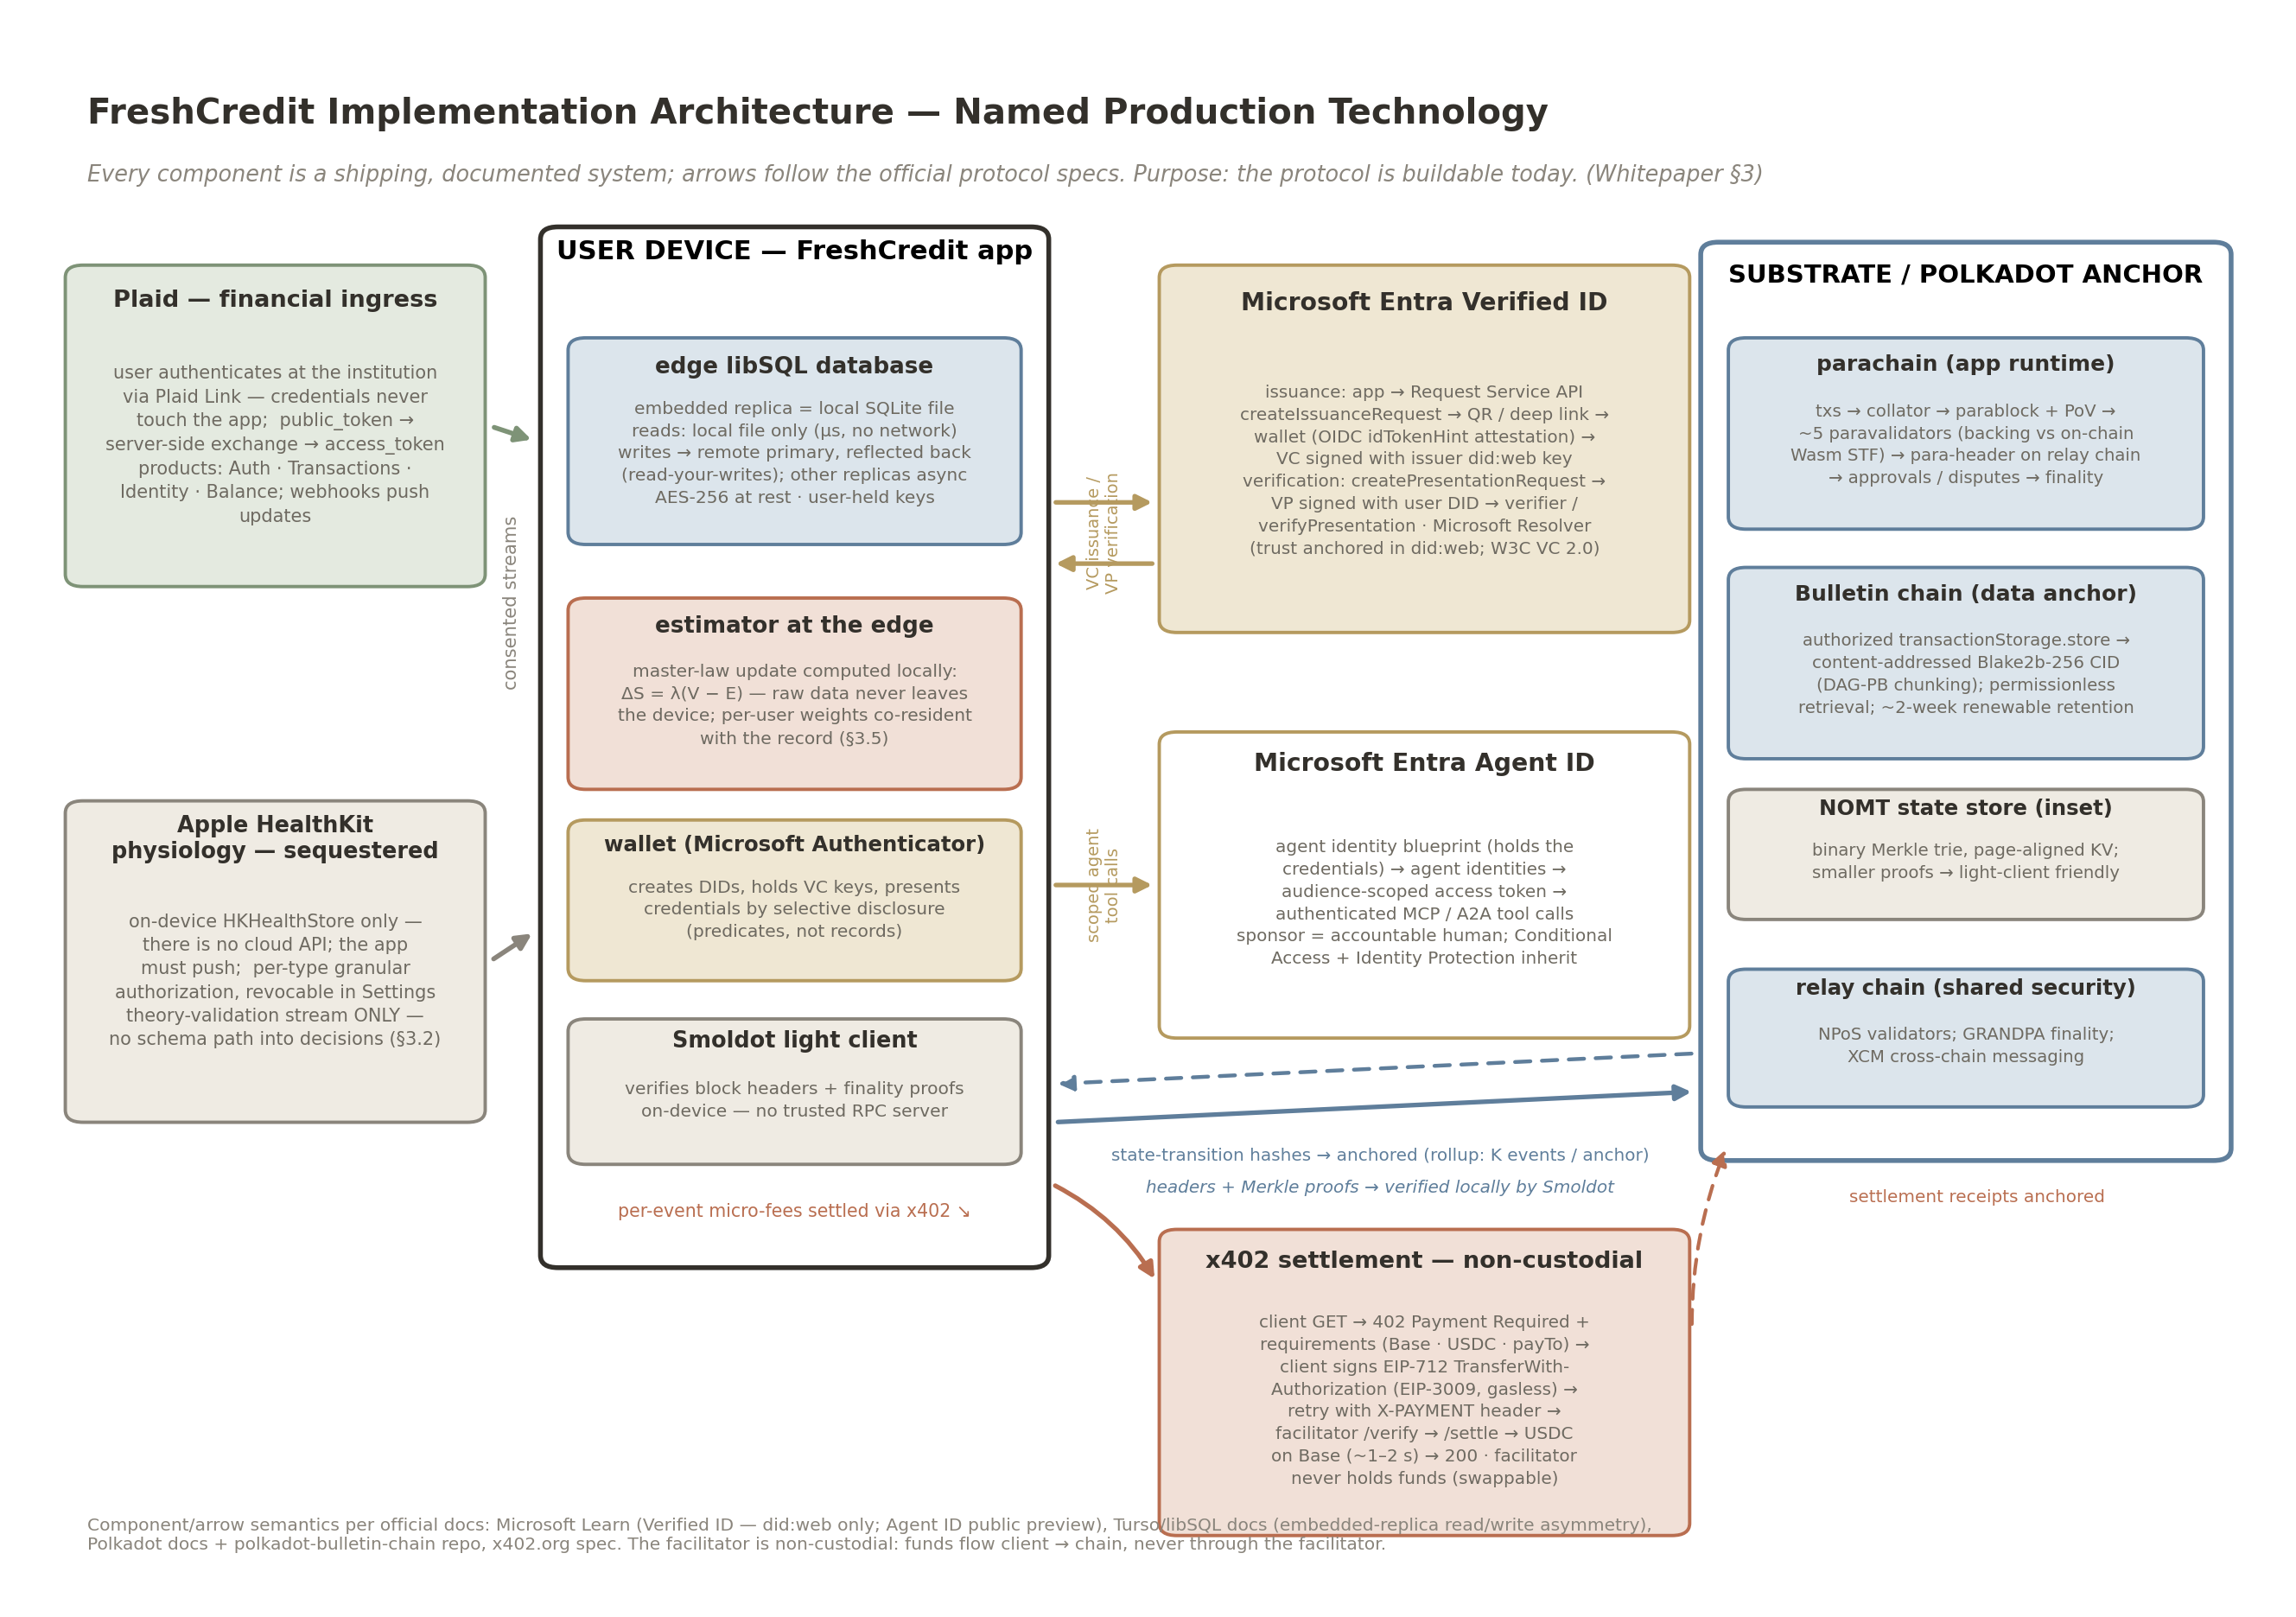
\includegraphics[width=\textwidth]{figures/wp_implementation_stack.png}
\caption{The FreshCredit implementation architecture with named production systems (\S~3): The companion measurement protocol unchanged at the core, configured for financial validation streams. Data ingress (left): Plaid (Link $\to$ public\_token $\to$ access\_token; Auth/Transactions/Identity/Balance products; webhooks --- user credentials never touch the app) and Apple HealthKit (on-device HKHealthStore only, per-type authorization, no cloud API; physiology sequestered from decisions). User device (center): the FreshCredit app holding the edge libSQL database (embedded replica; local $\mu$s reads, writes to the remote primary with read-your-writes, async other replicas, AES-256 at rest, user-held keys), the edge estimator computing $\Delta S = \lambda(V - E)$ locally, the Microsoft Authenticator wallet (DIDs, VC keys, selective disclosure), and the Smoldot light client (no trusted RPC). Identity (right-center): Microsoft Entra Verified ID (Request Service API issuance/verification flows, did:web trust anchor, Microsoft Resolver) and Entra Agent ID (blueprint $\to$ agent identity $\to$ audience-scoped token $\to$ MCP/A2A tool calls; sponsor + Conditional Access). Anchor (right): Substrate parachain block path (collator $\to$ parablock + PoV $\to$ paravalidators $\to$ relay chain, GRANDPA finality), Bulletin-chain content-addressed anchoring (Blake2b-256 CID, authorized store, $\sim$2-week renewable retention), NOMT state-store inset. Settlement: x402 (402 challenge $\to$ EIP-712/EIP-3009 gasless signature $\to$ X-PAYMENT retry $\to$ facilitator /verify + /settle $\to$ USDC on Base; facilitator non-custodial and swappable). \emph{Figure 1: implementation stack --- the protocol is buildable today from documented, production-grade components}}
\label{fig:wpstack}
\end{figure*}

\noindent\textbf{Figure 2.} The incumbent failure in regulator data (CFPB Consumer Response Annual Reports, 2025 and 2026 releases; CFPB Consumer Complaint Database; FCRA \S~611(e) report, December 2025). (a) Credit/consumer reporting is the dominant complaint category and rising: 85\% of all complaints received in 2024 ($\approx$2.70M of $\approx$3.19M), 88\% of a near-doubled total in 2025 (5,806,800 of 6,635,400); $\sim$93\% of credit-reporting complaints name the three nationwide bureaus. (b) Issue decomposition on the \emph{published-database} base (2,365,586 published credit-reporting complaints received in 2024): 49.7\% "incorrect information on your report" (1,175,009) + 19.3\% "problem with a company's investigation" (455,637) = 69.0\% error-related --- the database base differs from total receipts because not all complaints are published, and the shares do not transfer to the received base. (c) Trend: the incorrect-information issue's 2024 volume ran +247\% above the prior two years' monthly average; complaints against the three NCRAs ran roughly +3,000\% above January 2020 levels over January 2024--June 2025 --- raw intake-volume facts with the composition confound named: labels are self-classified, and the $\sim$3\% potentially-unauthorized-third-party flag bounds only unauthorized third parties (authorized dispute-mill volume is unbounded by it).

\emph{Figure 2: CFPB complaints}

\setcounter{figure}{2}% next float caption is Figure 3
\begin{figure*}[t!]
\centering
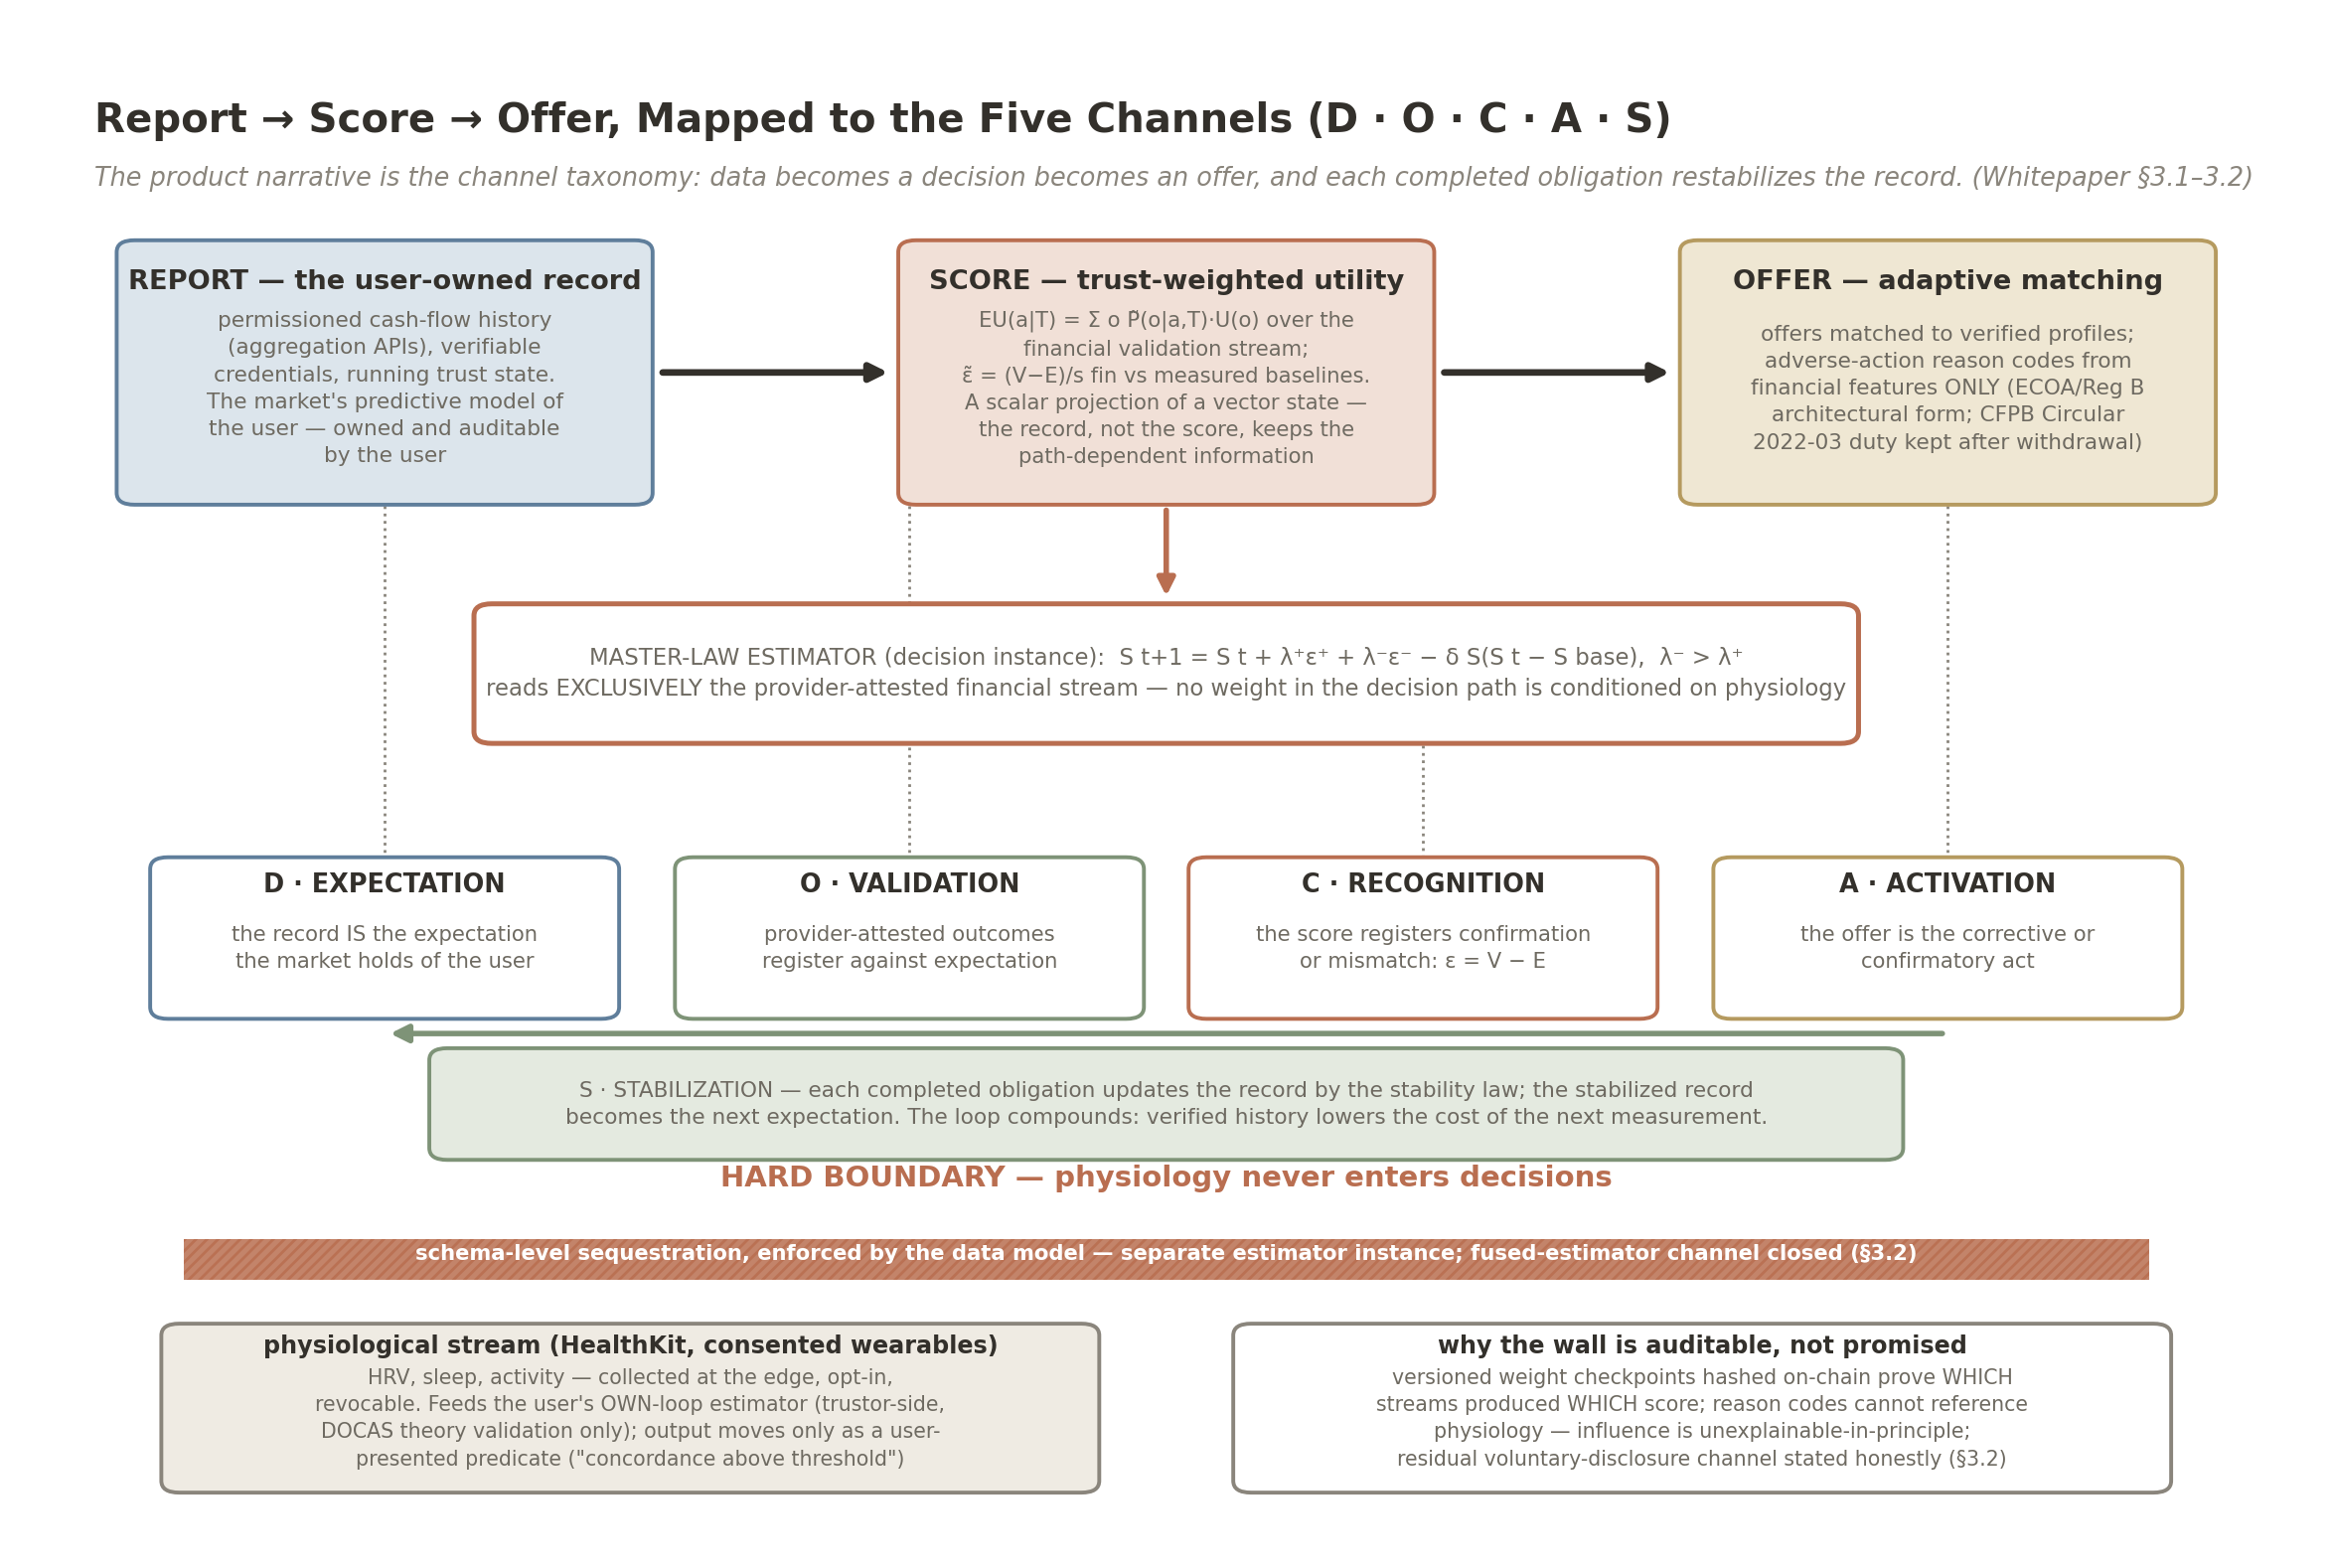
\includegraphics[width=\textwidth]{figures/wp_pipeline_channels.png}
\caption{Report $\to$ Score $\to$ Offer mapped to the five channels (\S~3.1--3.2). REPORT = D (Expectation): the user-owned record is the market's expectation of the user. SCORE = O (Validation) + C (Recognition): trust-weighted utility over the financial validation stream, registering confirmation or mismatch $\varepsilon = V - E$. OFFER = A (Activation): adaptive matching with adverse-action reason codes from financial features only. S (Stabilization) closes the loop: each completed obligation updates the record by the stability law and becomes the next expectation. The master-law estimator sits in the middle reading exclusively the provider-attested financial stream. Below the literal wall: the physiological stream (HealthKit/wearables) feeds only the user's own-loop (trustor-side) estimator for the companion biology preprint's theory validation; the boundary is schema-level, with on-chain weight-checkpoint audit and reason codes that cannot reference physiology --- physiology never enters decisions. \emph{Figure 3: the credit pipeline as the externalized biological loop, with the sequestration wall}}
\label{fig:wppipeline}
\end{figure*}

\begin{figure*}[t!]
\centering
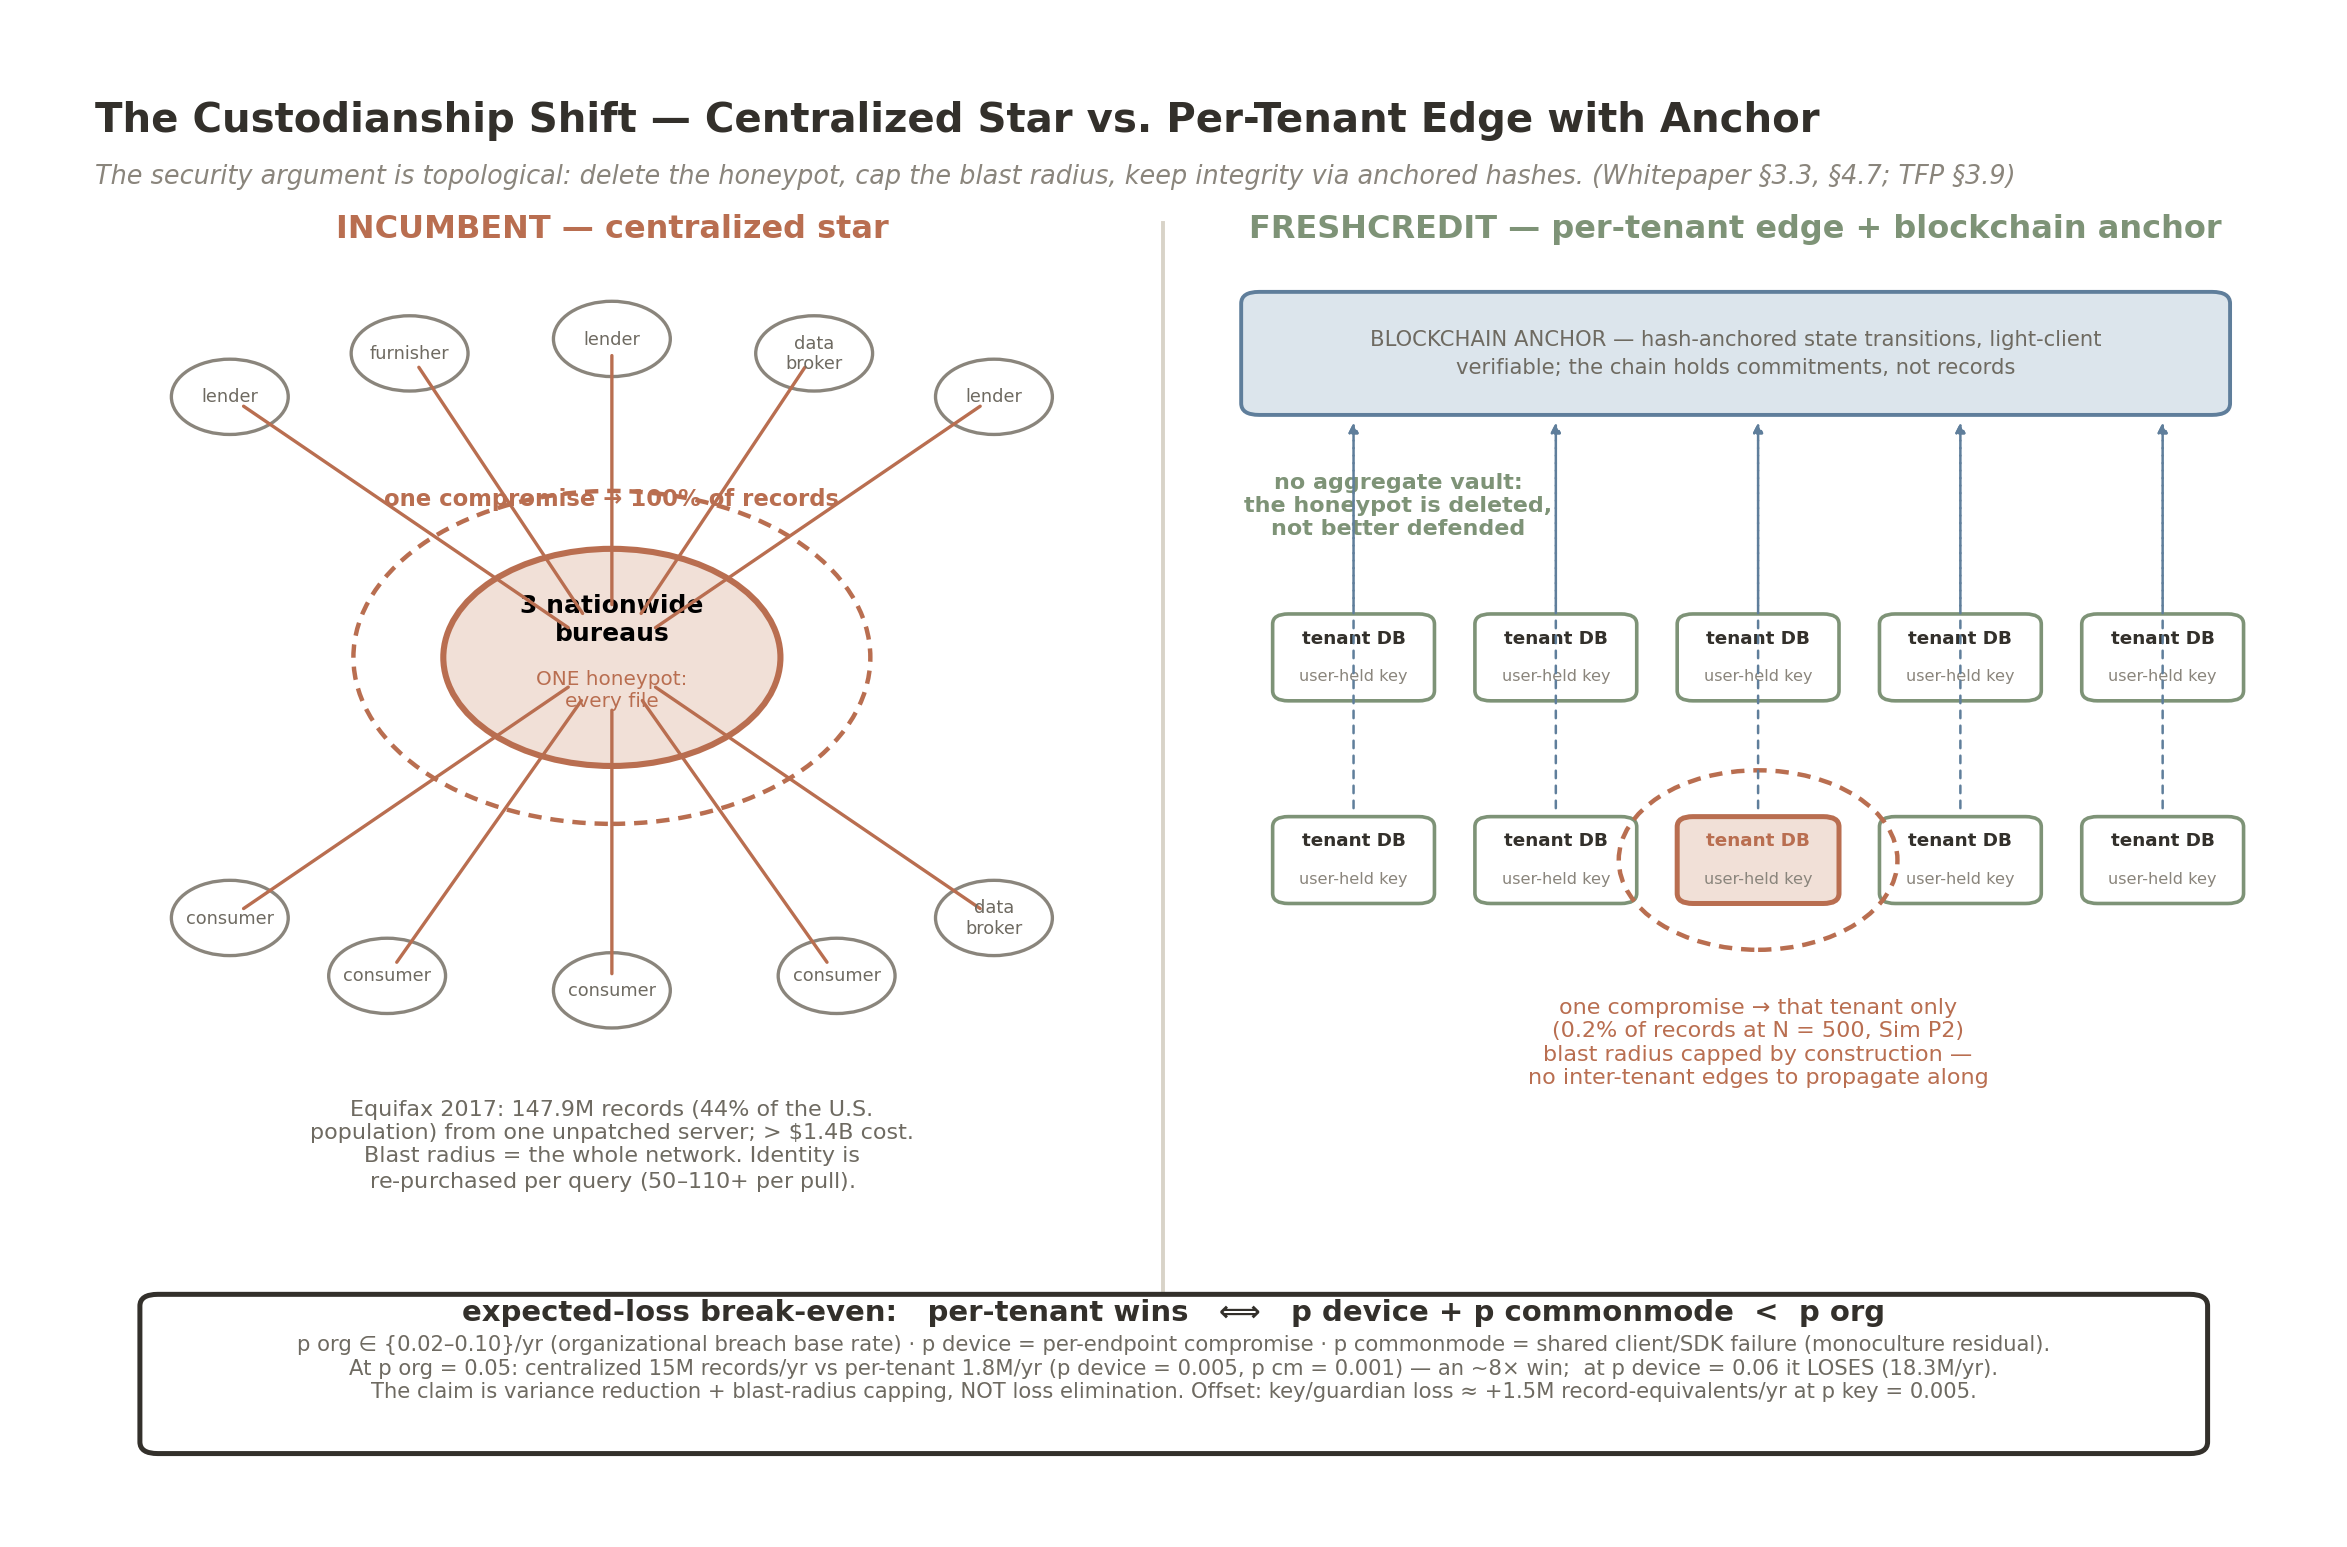
\includegraphics[width=\textwidth]{figures/wp_custodianship_shift.png}
\caption{The custodianship paradigm shift (\S~3.3; harm arithmetic in \S~4.3). Left: the incumbent centralized star --- three nationwide bureaus as a single honeypot; one compromise reaches 100\% of records (Equifax 2017: 147.9M records, $>$\$1.4B); identity re-purchased per query (\$50--\$110+ per pull). Right: per-tenant edge databases with user-held keys under a blockchain anchor --- local immutability via hash-anchored state transitions, no aggregate vault, blast radius capped at the breached tenant by construction (0.2\% at $N = 500$, the companion protocol preprint's Sim P2, conditional on a breach). Inset: the expected-loss break-even $p_{\mathrm{device}} + p_{\mathrm{commonmode}} < p_{\mathrm{org}}$ with anchors (at $p_{\mathrm{org}} = 0.05$: 15M vs 1.8M records/yr, $\sim$8$\times$ win in the favorable region; loss at $p_{\mathrm{device}} = 0.06$), the headline (variance reduction and blast-radius capping, not loss elimination), and the key/guardian-loss offset ($\sim$+1.5M record-equivalents/yr at $p_{\mathrm{key}} = 0.005$). No DebtRank-form cascade panel is shown (companion protocol preprint, Sim P6: category error for data custody). \emph{Figure 4: two architectures, two risk geometries}}
\label{fig:wpcustody}
\end{figure*}

\begin{figure*}[t!]
\centering
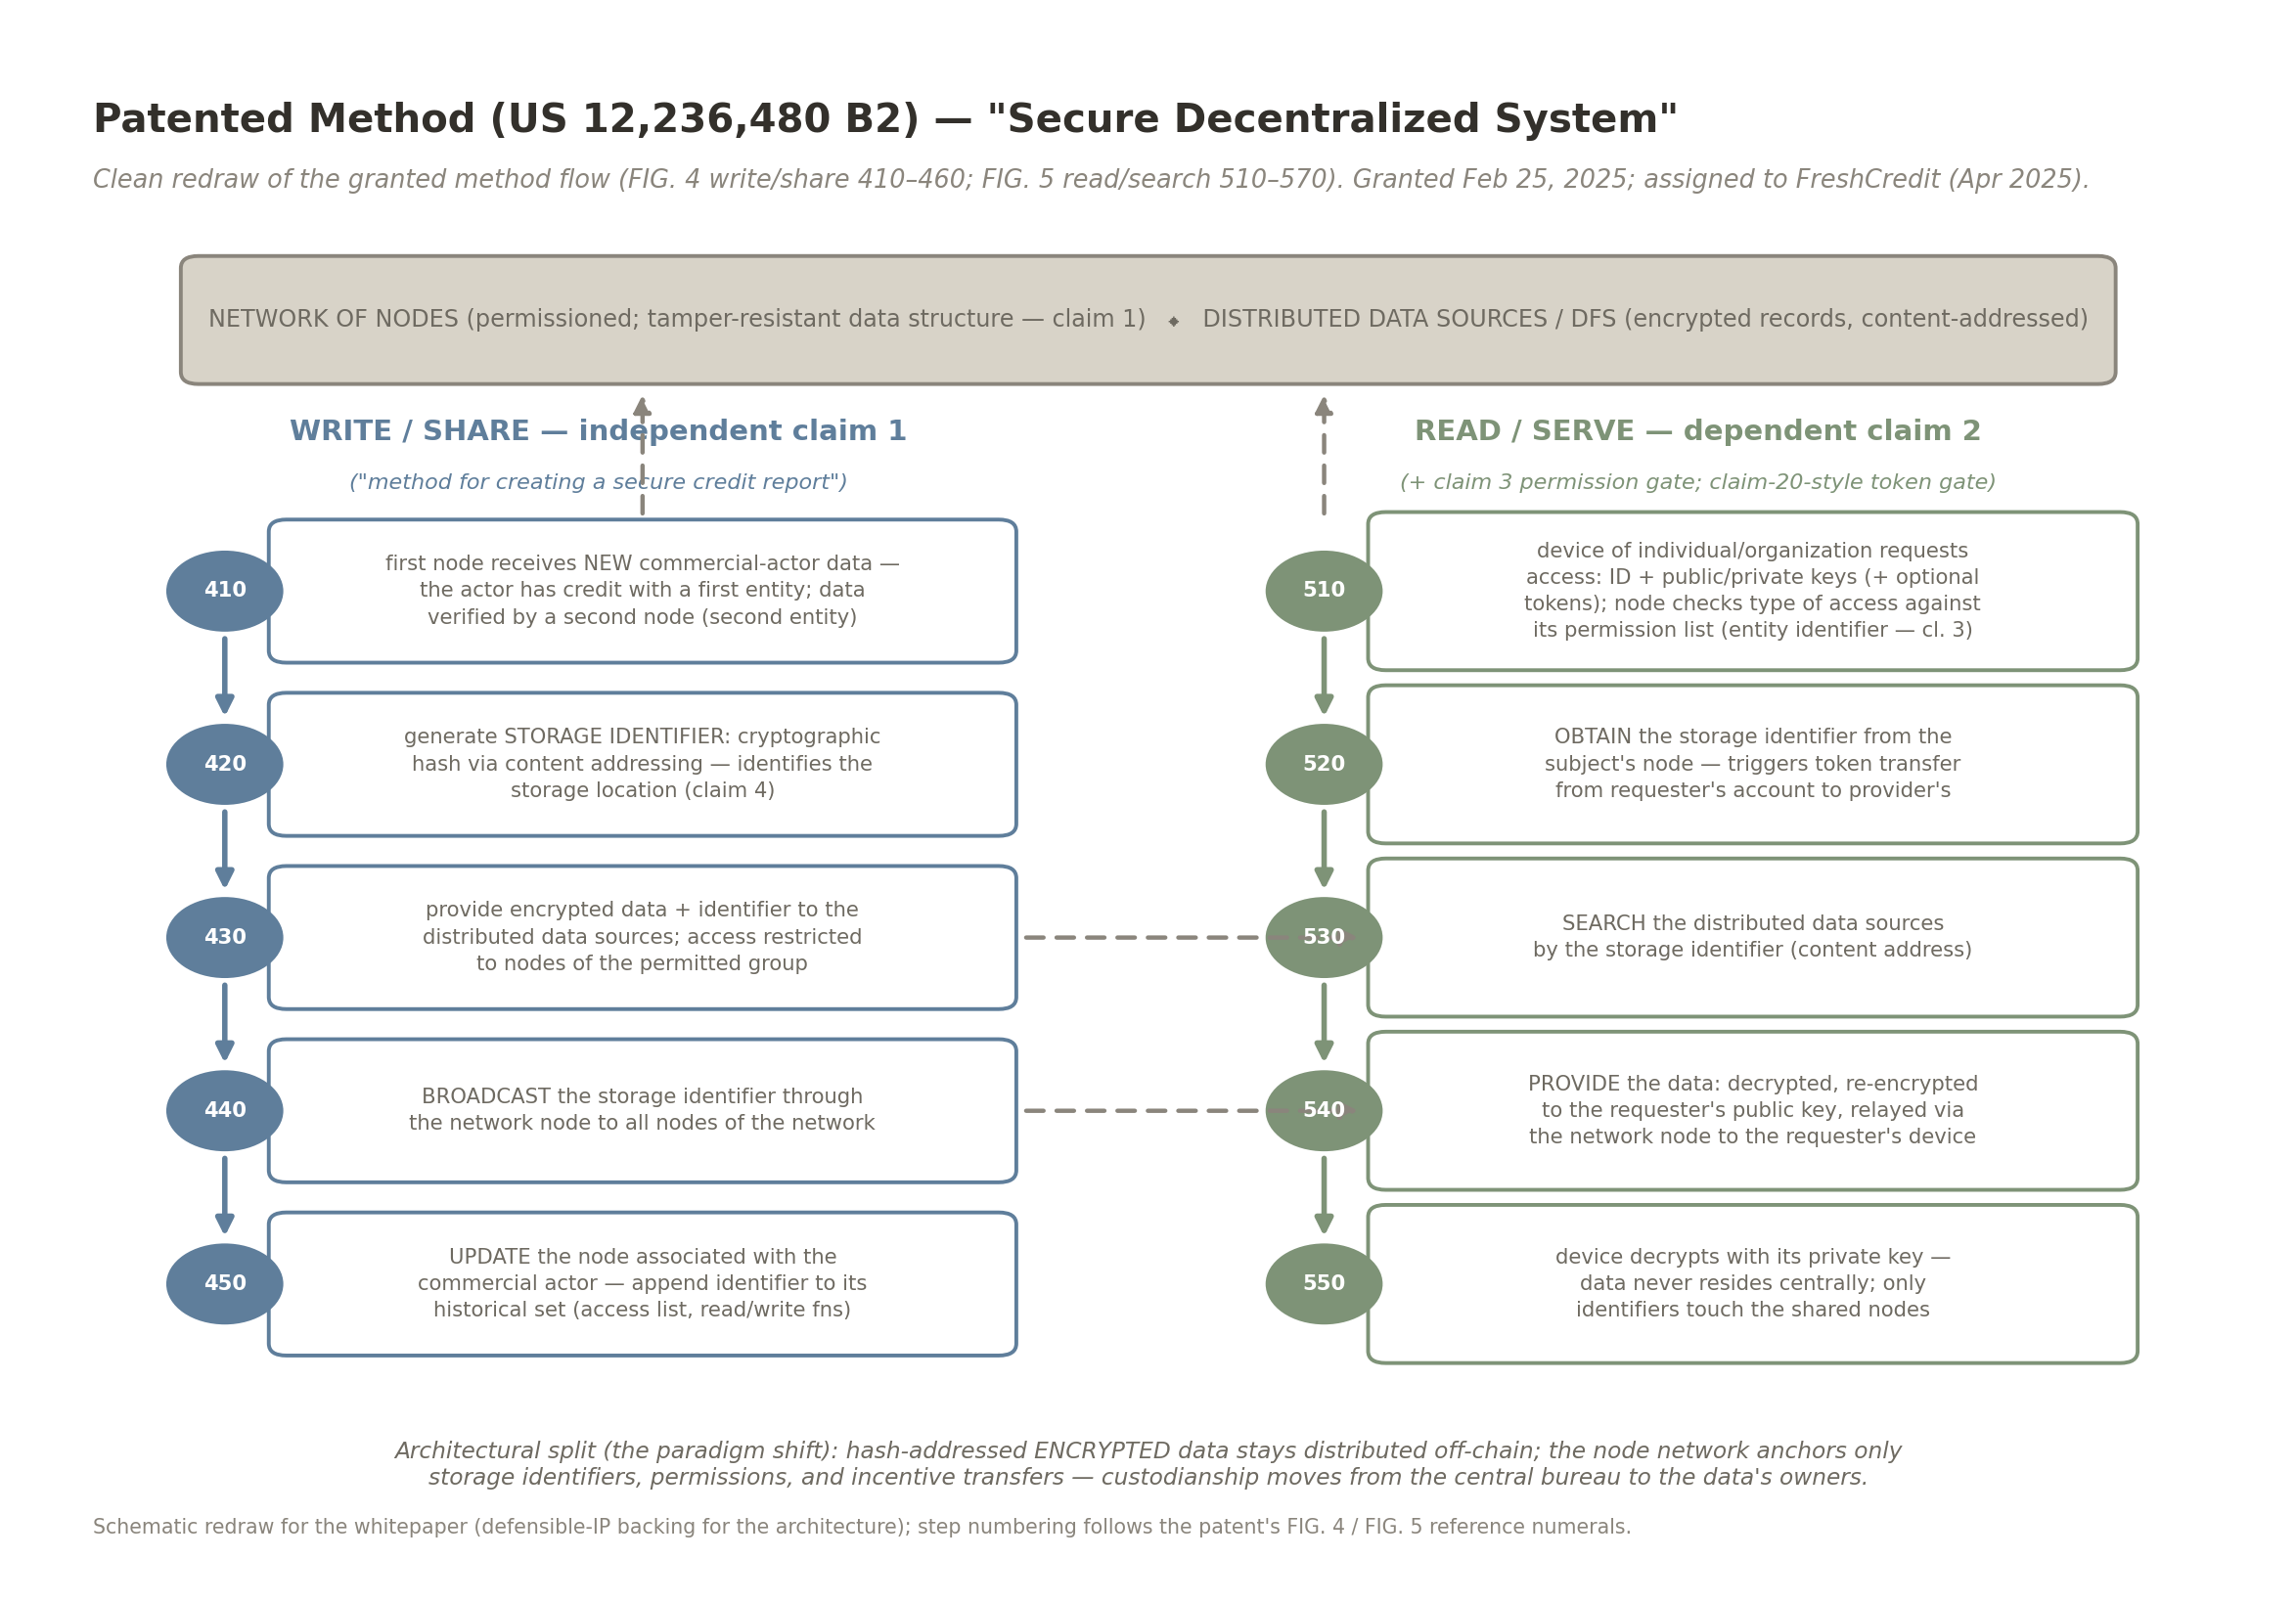
\includegraphics[width=\textwidth]{figures/wp_patented_method_flow.png}
\caption{The patented method behind the custodianship shift (\S~4.2; US 12,236,480 B2, ``Secure Decentralized System,'' granted February 25, 2025 \citep{shigaki2025us12236480}; assigned to FreshCredit, April 2025; divisionals granted as US 12,293,410 B2 and US 12,307,515 B2, May 2025 \citep{shigaki2025us12293410,shigaki2025us12307515}; fourth family grant US 12,293,411 B2 \citep{shigaki2025us12293411} --- grant statuses per public records). Write/share lane (independent claim 1, ``method for creating a secure credit report''): a first node receives new, second-node-verified commercial-actor data (410); generates a content-addressed cryptographic-hash storage identifier (420; claim 4); provides encrypted data + identifier to the distributed data sources under the tamper-resistant, permissioned structure (430); broadcasts the identifier through the network of nodes (440); and updates the commercial actor's node (450). Read/serve lane (dependent claim 2, with the claim-3 permission gate and claim-20-style token gate; the patent's FIG.~5 steps 510--570 compressed to five steps preserving order and content): device request with ID + keys (510); obtain the storage identifier from the subject's node, triggering the requester $\to$ provider token transfer (520); search the distributed data sources by content address (530); provide the data re-encrypted to the requester's public key (540); the device decrypts locally (550). The architectural split --- encrypted data distributed off-chain, nodes anchoring only identifiers/permissions/incentives --- is the patented basis of the custodianship shift. \emph{Figure 5: patented method flow (redrawn from the patent's FIG.~4/FIG.~5)}}
\label{fig:wppatent}
\end{figure*}

\begin{figure*}[t!]
\centering
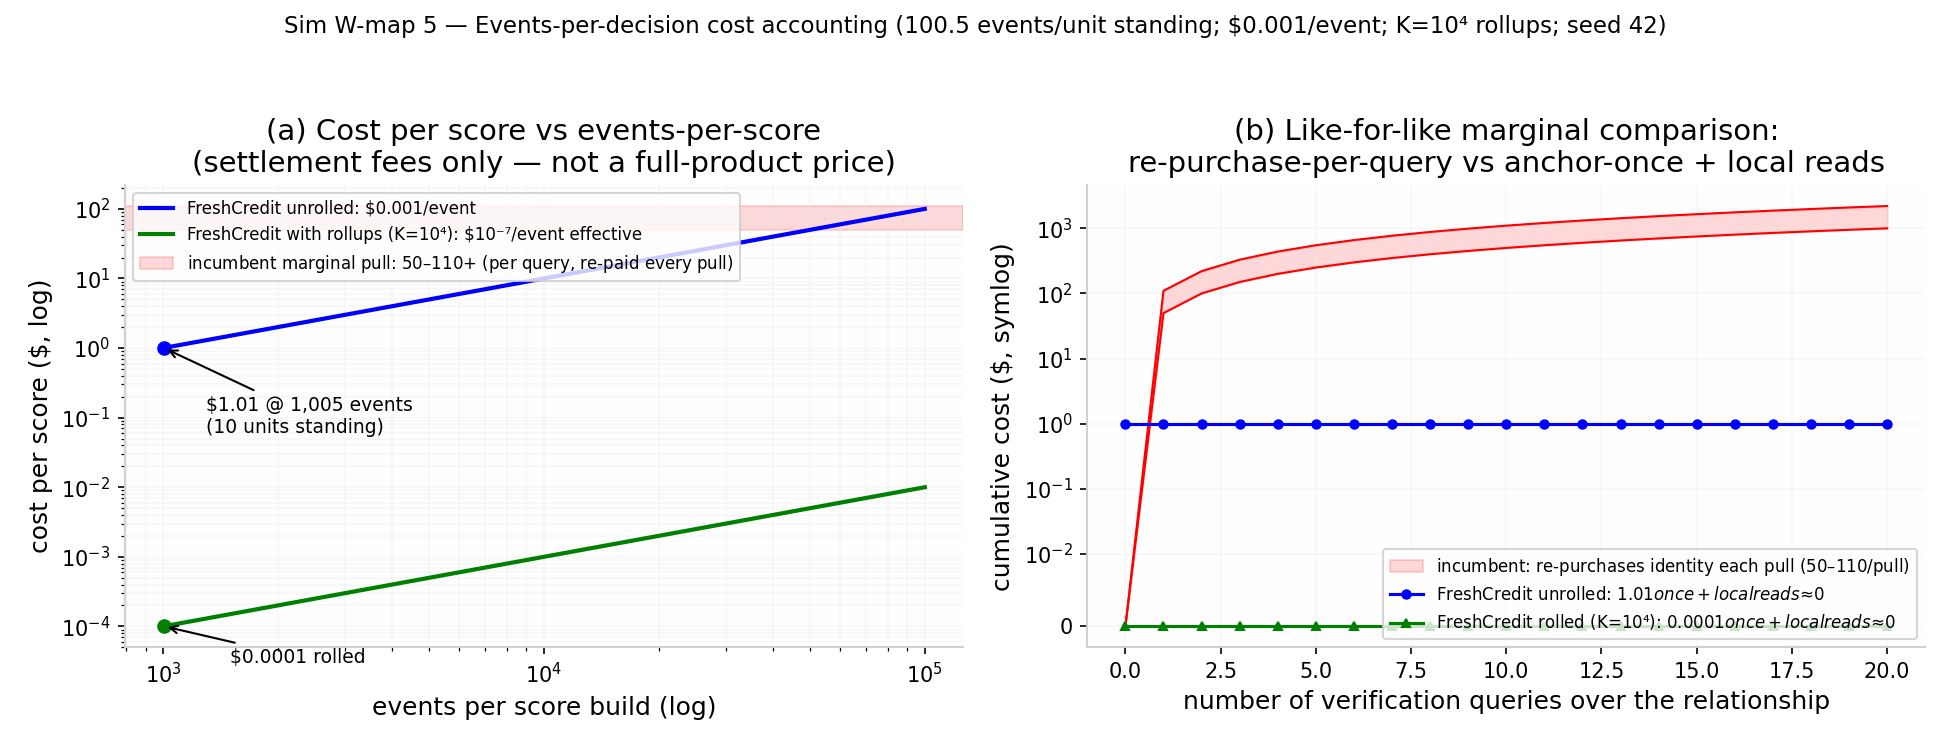
\includegraphics[width=\textwidth]{figures/figW5_cost_accounting.png}
\caption{The cost of manufactured history is time, not money --- and the honest user's cost is decoupled from both (Technical Appendix, Sim-Battery A, Study 3; Sim W5). The Sybil-side numbers, carried in \S~1.4: without provider attestation \$1.01 buys 10 units of standing (the "costly to fake" claim is false in money); attestation multiplies cost linearly in the multiplier m but is a weak deterrent at m $\leq$ 10; the real defense is the wall-clock time floor, quoted per rate --- manufacturing 10 units takes 5.5/2.8/1.4 years at 0.5/1/$\leq$2 attested events/day and $\sim$0.55--1.1 years at the model's own high-standing rates (2.5--3.76 events/day, 5/day max grid; 0.73 yr at 3.76/day; 0.55 yr at 5/day) --- with the parallel-provider-collusion caveat carried in-paper. The rendered panels price the honest side: (a) anchoring cost per unit of standing vs. events per score ($10^{3}$--$10^{5}$), unrolled ($\sim$\$0.001/event) vs. rolled ($K = 10^{4}$ events/anchor), against the incumbent per-pull band (\$50--\$110+): the lifetime $\sim$1,005-event history anchors for \$1.005 unrolled and \$0.0001 rolled --- a $10^{4}\times$ discount that does not touch the Sybil time floor; (b) cumulative cost over repeated verification queries --- the incumbent re-purchases identity at every query while the anchored identity's reads are local ($\approx$\$0). \emph{Figure 6: Sybil cost, the wall-clock defense, and honest-side cost accounting (whitepaper battery figure figW5; figure in the Supporting Document deposit)}}
\end{figure*}

\begin{figure*}[t!]
\centering
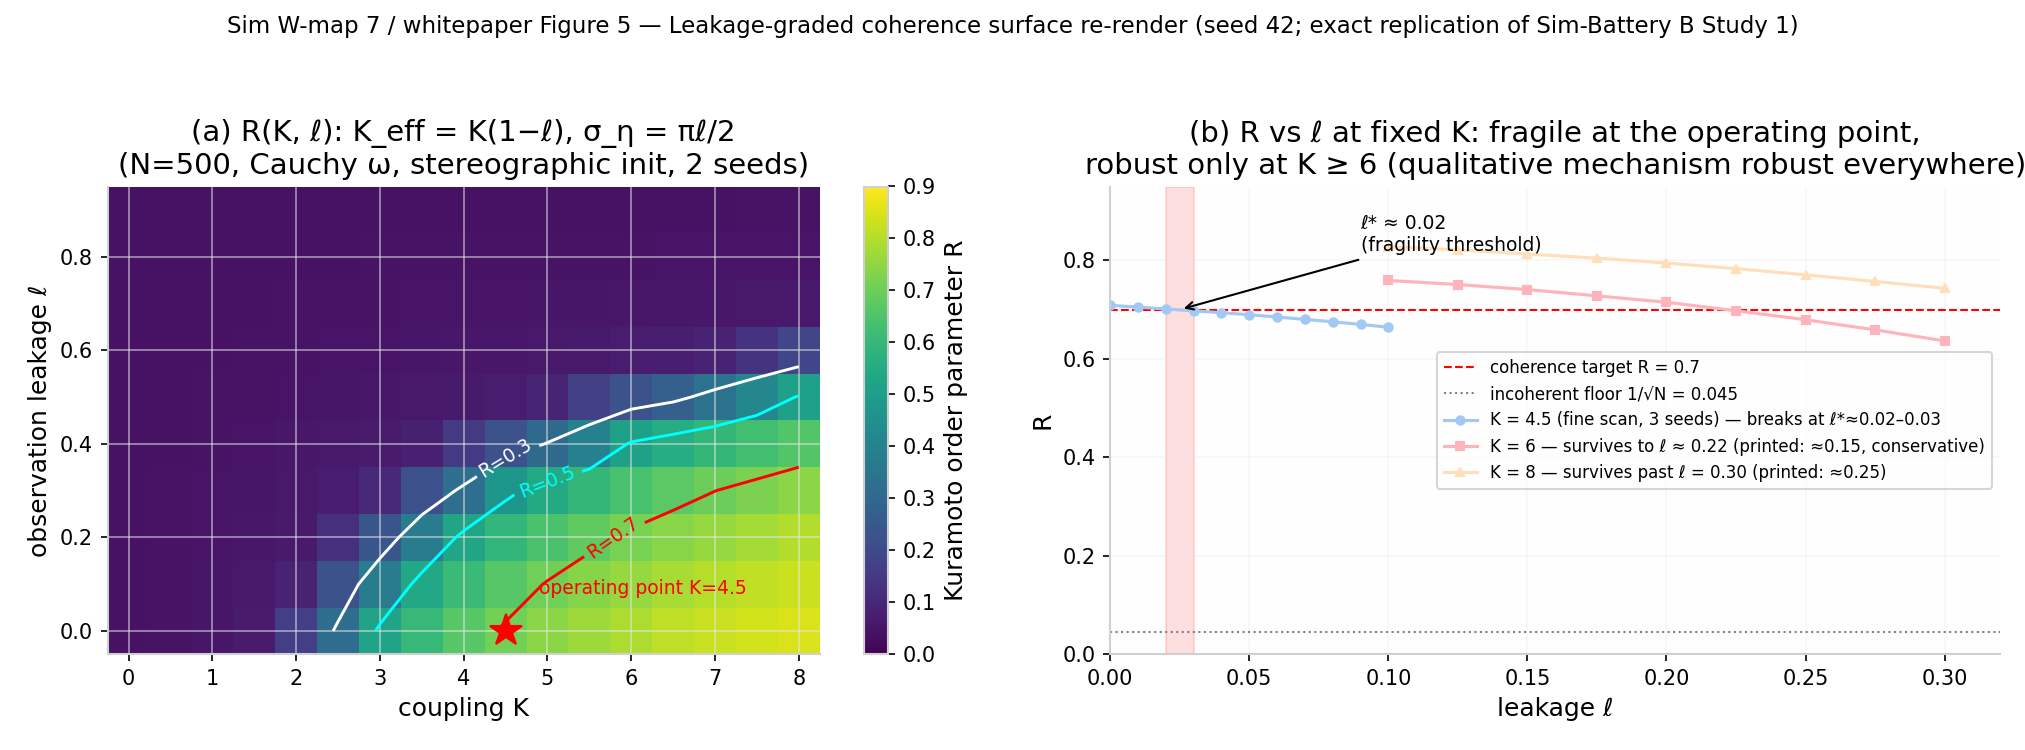
\includegraphics[width=\textwidth]{figures/figW7_R_surface.png}
\caption{Coherence requires coupling \emph{and} low leakage (Technical Appendix, Sim-Battery B, Study 1). (a) Kuramoto order parameter R over coupling K $\in$ [0, 8] $\times$ observation leakage $\ell$ $\in$ [0, 0.9] (N = 500, Cauchy frequencies, stereographic phase initialization; $K_{\mathrm{eff}} = K(1-\ell)$, $\sigma_{\eta} = \pi\ell/2$): R rises from the $1/\sqrt{N}$ floor to $\approx$ 0.85 at K = 8, $\ell$ = 0, and the R = 0.7 contour retreats from K $\approx$ 4.4 ($\ell$ = 0) to K $\approx$ 5.0--5.5 ($\ell$ = 0.1) and K $\approx$ 5.9--7 ($\ell$ = 0.2), moving off-grid for $\ell$ $\gtrsim$ 0.25--0.4 across re-renders (ranges span two independent seeded re-renders; point precision is not resolvable at these N). (b) R vs. $\ell$ at fixed K. At the K = 4.5 operating point the fragility crossing is a band $\ell^{*}$ $\in$ [0.02, 0.10]; at K = 6 coherence survives to $\ell$ $\approx$ 0.22--0.28 and at K = 8 to $\ell$ $\approx$ 0.30--0.40. A half-circle (arctan) phase map would inflate the K = 0 control to R $\approx$ 0.635; the incoherent baseline under the stereographic map is $\approx$ 0.03--0.05. $\ell$ is a model-internal parameter with no field operationalization yet. \emph{Figure 7: Leakage-graded coherence surface (whitepaper battery re-render figW7 of figB1\_R\_surface.png; figure in the Supporting Document deposit)}}
\end{figure*}

\begin{figure*}[t!]
\centering
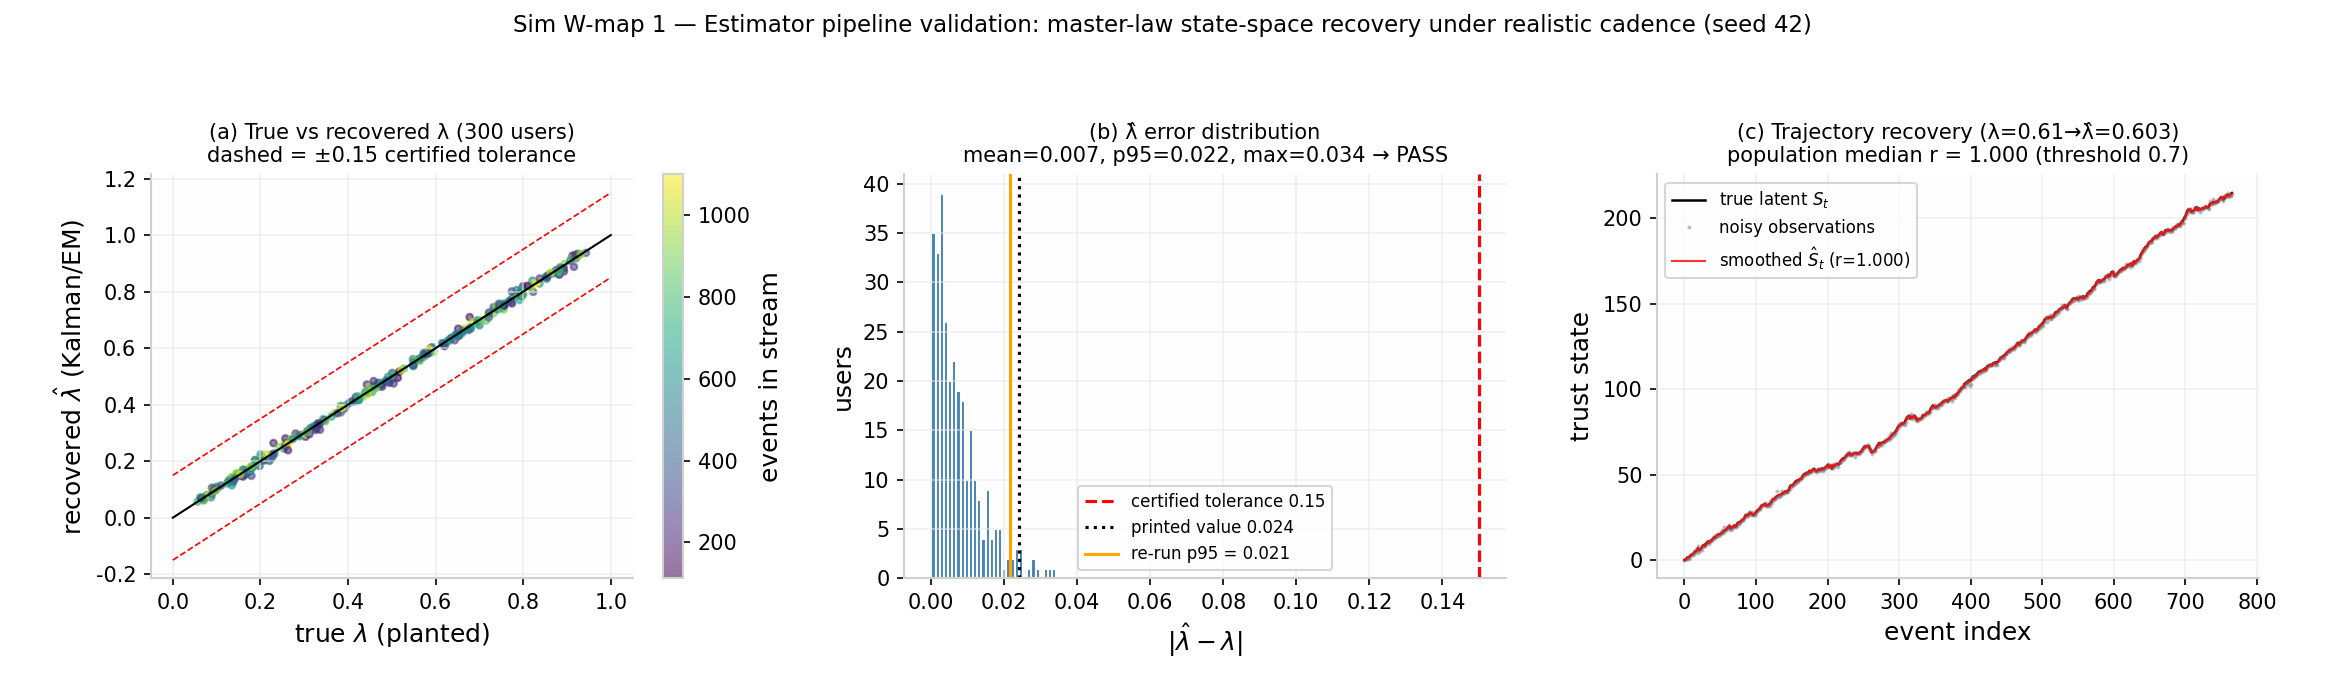
\includegraphics[width=\textwidth]{figures/figW1_estimator_validation.png}
\caption{Estimator validation on synthetic ground truth (Sim W2; \S~3.4). 300 synthetic users, true $\lambda \sim \mathrm{U}[0.05, 0.95]$, mixed-sign $\tilde{\varepsilon}$ streams (12--15\% negative, heavier-tailed betrayals), Poisson cadence 0.3--3.0 events/day over 365 days (median 569 events/user, range 112--1100), heavy-tailed Student-t observation noise, and a deliberately misspecified Kalman/EM estimator. (a) True vs. recovered $\hat{\lambda}$ with the $\pm$0.15 certified band; (b) recovery-error histogram against the certified tolerance 0.15 and the printed 0.024 --- re-run |$\hat{\lambda}$ - $\lambda$|: mean 0.0074, p95 0.0215, max 0.0343; planted $\lambda$ = 0 negative control max|$\hat{\lambda}$| = 0.0092; ultra-thin streams (60--110 events) max error 0.0737; (c) example latent-trajectory recovery (single-stream scope; median r = 1.000 --- see the \S~3.4 scope note). \emph{Figure 8: Estimator validation (whitepaper battery figure figW1)}}
\end{figure*}

\begin{figure*}[t!]
\centering
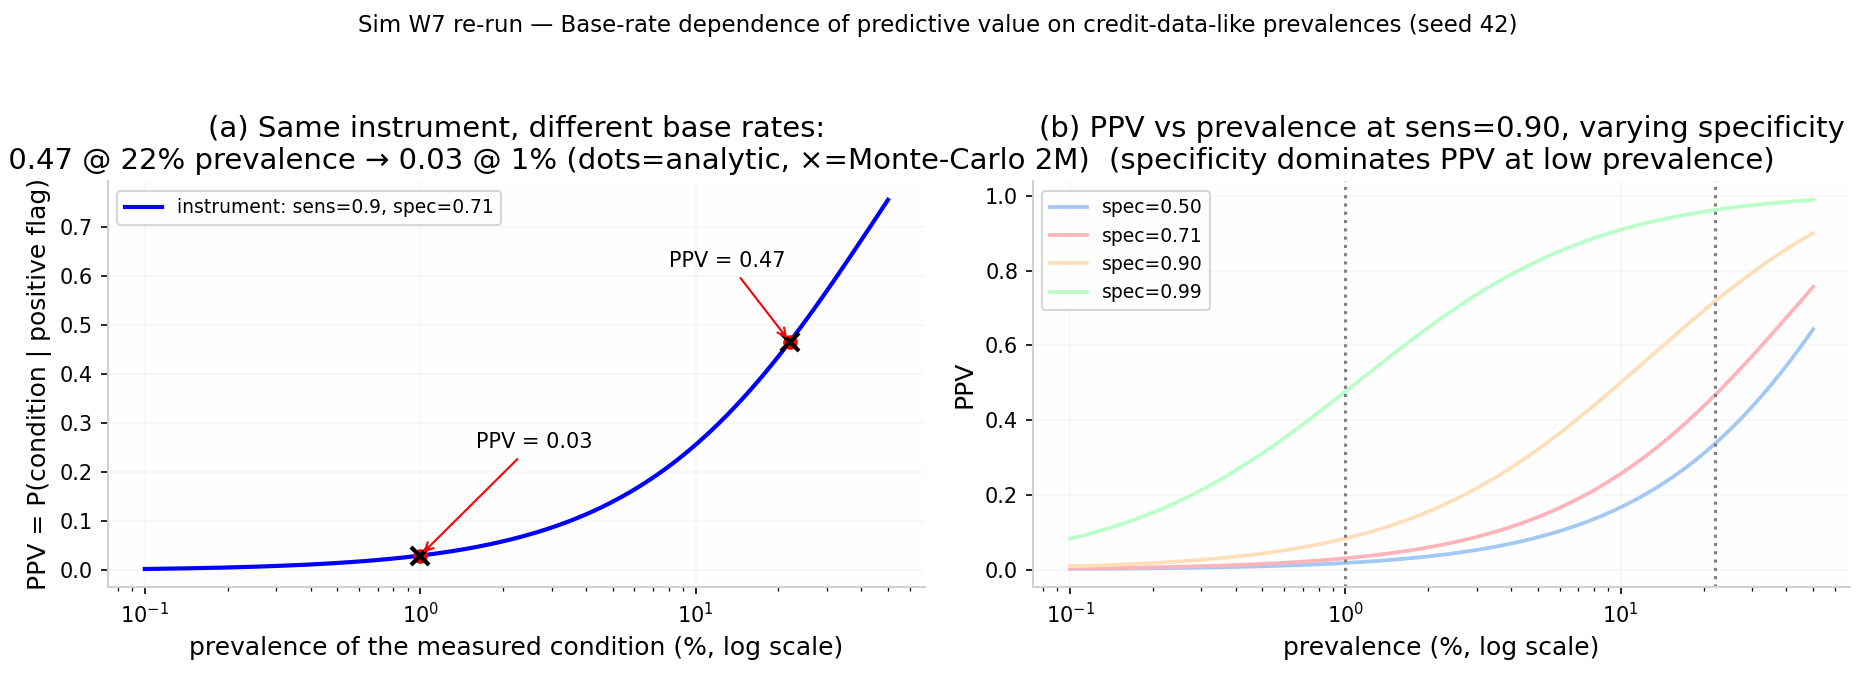
\includegraphics[width=\textwidth]{figures/figW2_ppv_baserate.png}
\caption{Base-rate dependence of predictive value (Sim W1 re-run; \S~1.5). Same instrument (sensitivity 0.90, specificity 0.71 --- an assumed instrument operating point, stated for the base-rate illustration), $\approx$15$\times$ PPV collapse purely from the base rate (0.4668/0.0304 = 15.4$\times$). (a) PPV vs. prevalence: 0.47 at 22\% prevalence falling to 0.03 at 1\% --- analytic values and Monte-Carlo crosses (2M files, seed 42) coincide with the printed points. (b) PPV vs. prevalence at sensitivity 0.90 across specificities: specificity, not sensitivity, dominates PPV at low prevalence. \emph{Figure 9: PPV vs. base rate (whitepaper battery figure figW2)}}
\end{figure*}

\begin{figure*}[t!]
\centering
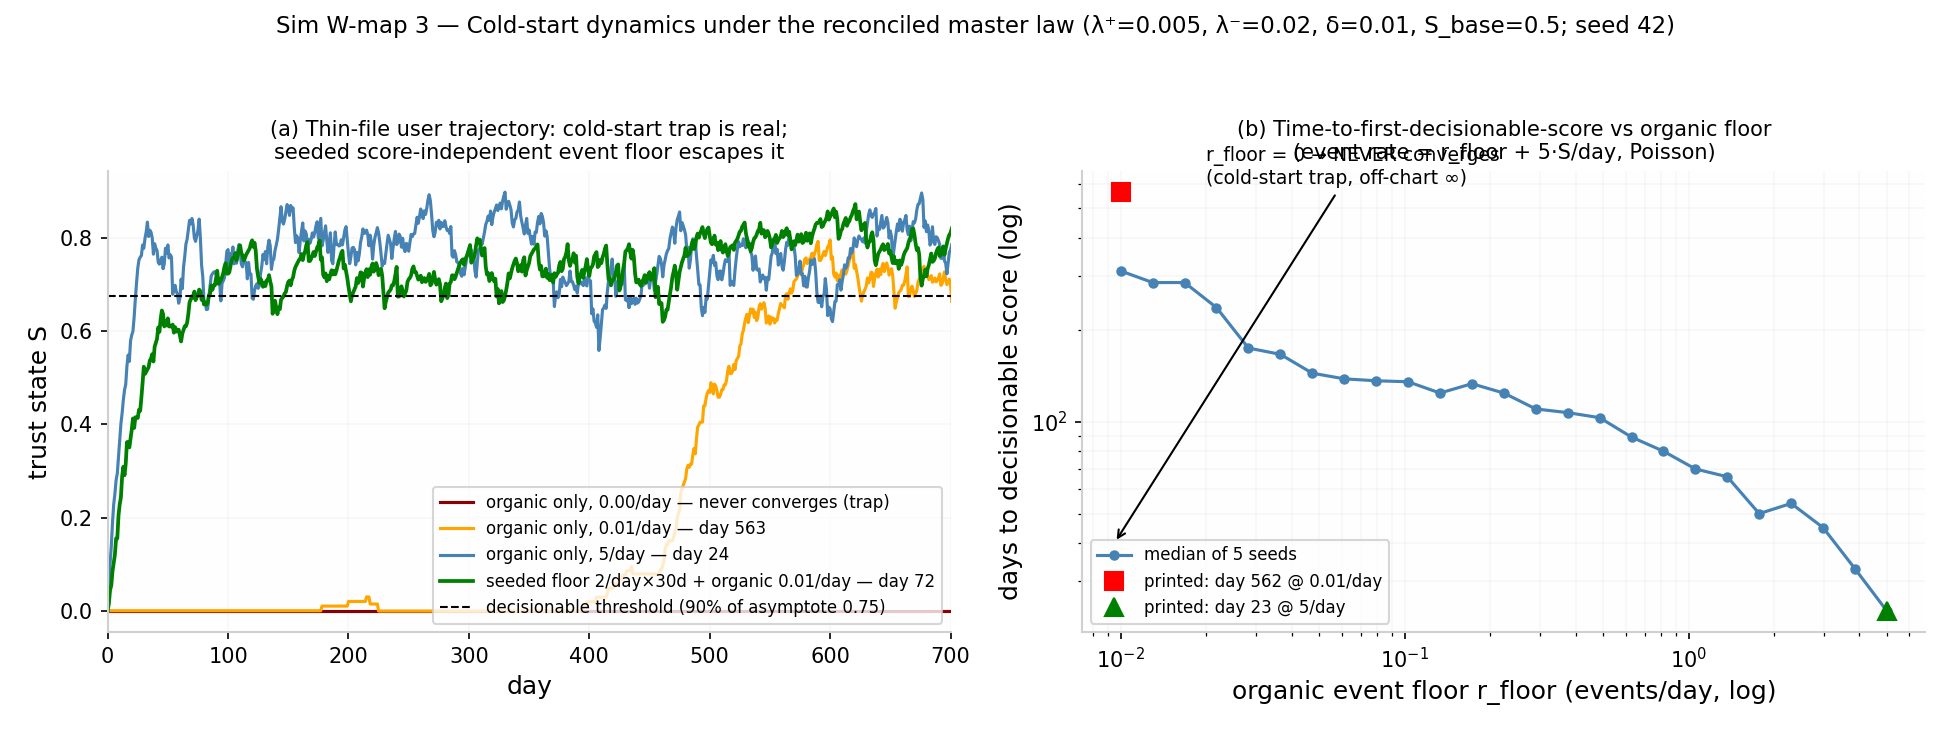
\includegraphics[width=\textwidth]{figures/figW3_coldstart.png}
\caption{The cold-start trap and the seeded-floor escape (Sim-Battery A, Study 1 re-run; \S~4.3 channel 4). (a) Trust-state trajectories S(t): with zero organic floor the new user never converges (the trap); two convergence criteria, both verified --- first-crossing ($S \geq 0.9\,S^*$, $S^* = 0.75$) reaches a decisionable score at day $318 \pm 133$ at 0.01 organic events/day (189/149/112/76/30 days at 0.05/0.1/0.5/1/5 per day) and stabilization-to-asymptote at days 563/144/140/120/72/24 across the same floor grid; the earlier single-grid printing conflated the two criteria. A seeded score-independent floor of 2 events/day for 30 days escapes at day 72 --- 4.4$\times$ versus first-crossing and 7.8$\times$ versus stabilization on the organic-only 0.01/day clock. (b) Time to first decisionable score vs.\ organic floor (median of 5 seeds) under the first-crossing criterion. \emph{Figure 10: Cold-start trajectories (whitepaper battery figure figW3)}}
\end{figure*}

\begin{figure*}[t!]
\centering

\includegraphics[width=\textwidth]{figures/figW4_adoption_compounding.png}
\caption{Adoption compounding with densification feedback (Sim W3; \S~4.1). Adoption ODE with densification coupling $\zeta$ feeding back through the cold-start clock of Figure 10. (a) Adopted fraction after 10 years over (organic floor $\times$ $\zeta$): the stall region (floor $\lesssim$ 0.01/day \textbf{and} $\zeta$ $\lesssim$ 0.5; adopted fraction $<$ 0.2), the compounding region (floor $\geq$ $\sim$0.1/day, or $\zeta$ $\geq$ $\sim$2, or strong densification alone; $\geq$ 0.8), and the exact trap only at $(\mathrm{floor},\, \zeta) = (0, 0)$. (b) Representative trajectories: trap, stall, partial, compound, and the densification-only arm --- $\zeta$ = 5 with zero organic floor bootstraps off the 1\% initial cohort to $\sim$95\% by year 10, the modeling-choice caveat carried in \S~4.1. \emph{Figure 11: Adoption phase diagram (whitepaper battery figure figW4)}}
\end{figure*}

\begin{figure*}[t!]
\centering
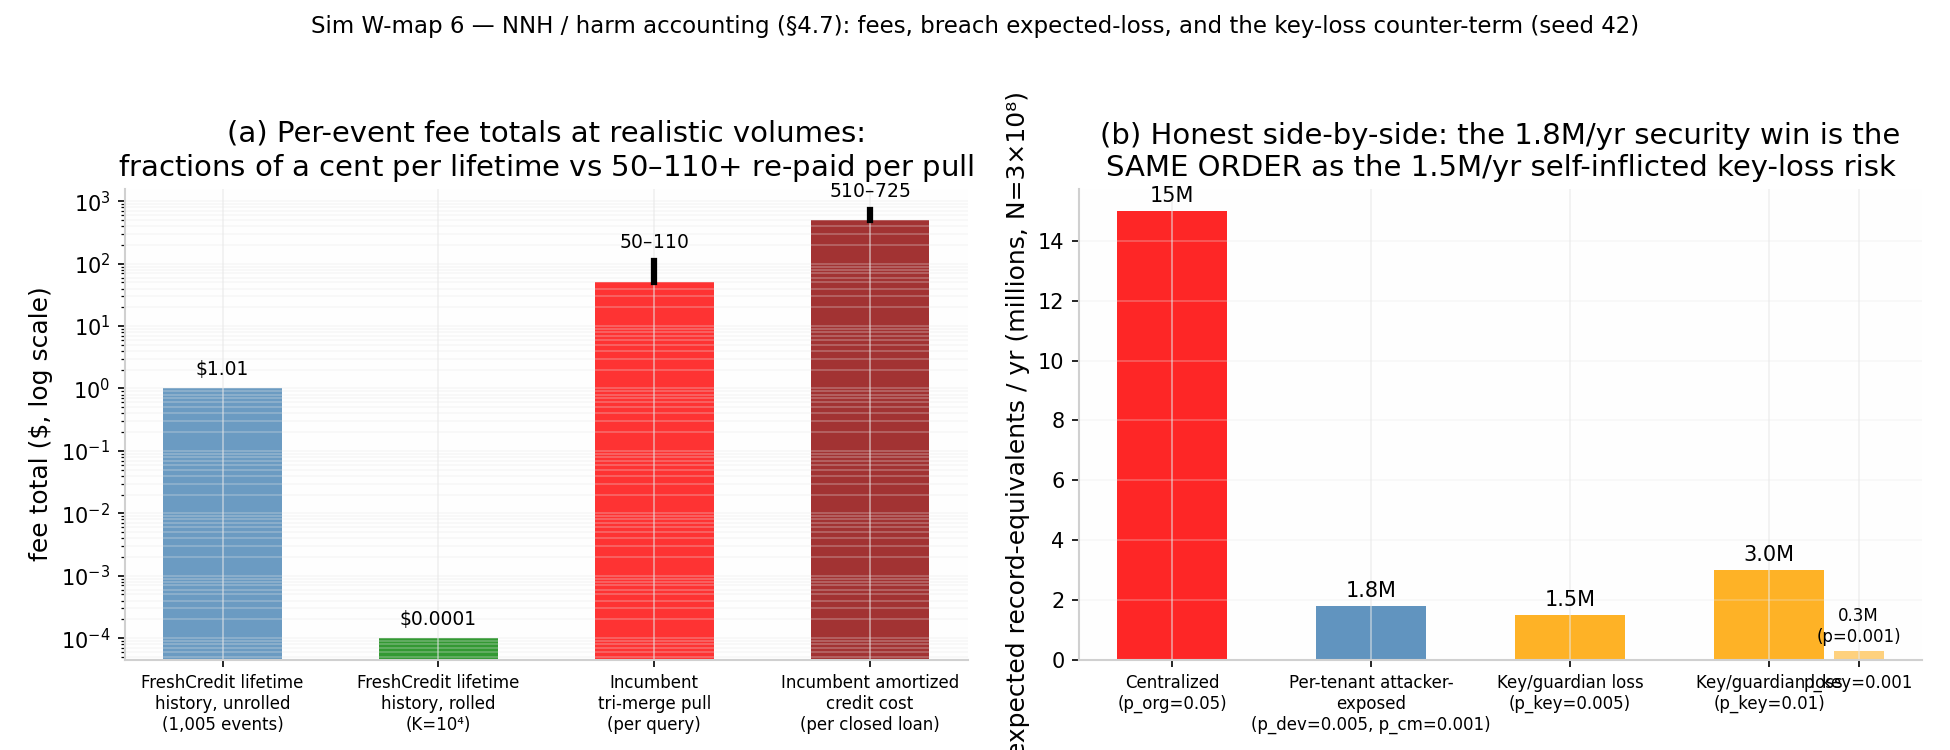
\includegraphics[width=\textwidth]{figures/figW6_nnh_harm.png}
\caption{Number-needed-to-harm accounting (Sim W4; \S~4.3). (a) Fee totals (log scale): fractions of a cent per lifetime --- \$1.005 unrolled, \$0.0001 rolled for a full $\sim$1,005-event history --- with provider-attestation cost at multiplier m (\$10.05/\$100.50/\$1,005 per 10 units at m = 10/100/1,000) the dominant fee channel; the like-for-like incumbent comparison is carried in \S~4.1. (b) Records per year: centralized expected exposure 15M/yr ($p_{\mathrm{org}}$ = 0.05, $3\times 10^{8}$ tenants), per-tenant attacker-exposed 1.8M/yr (8.3$\times$ reduction), and the key/guardian-loss counter-term 0.3 / 1.5 / 3.0M/yr at $p_{\mathrm{key}}$ = 0.001 / 0.005 / 0.01 --- the security win and the availability offset printed side by side. \emph{Figure 12: NNH --- the win and the counter-term (whitepaper battery figure figW6)}}
\end{figure*}

\clearpage
\bibliographystyle{plainnat}
\nocite{*}
\bibliography{whitepaper}

\vspace{1em}\begin{footnotesize}
\emph{Live benchmarks (supplementary): freshcredit.xyz/cost. Modeled projections are labeled as such; no production performance is claimed; nothing in this document is an offer of credit or a commitment to lend.}
\end{footnotesize}
\end{document}
